% *******************************************************************
% STOP - Bitte zuerst lesen, bevor Sie weitermachen
%
% Einige Dinge müssen Sie an Ihre Bedürfnisse (und die Vorgaben Ihres
% Betreuers anpassen).
%
% 1. Sprache
% Das Template unterstützt Deutsch und Englisch, Standard ist Deutsch.
% Wenn Sie Englisch verwenden wollen, ändern Sie bitte direkt am Anfang
% dieser Datei den Eintrag
%    \newcommand{\hsmasprache}{de}
% auf
%    \newcommand{\hsmasprache}{en}
%
% 2. Zitierstil
% Abhängig von dem gewünschten Zitierstil passen Sie bitte in
% preambel.tex die Einstellungen bei \usepackage[backend=biber...
% an. Wie ist dort genau erklärt.
% Achtung: Wenn Sie als Zitierstil Fußnoten wählen bzw. generell
% -------  mit Fußnoten arbeiten, dann beachten Sie bitte, dass
%          Fußnoten in Bildunterschriften und Tabellenüberschrifte
%          nicht funktionieren.
%          Siehe hierzu https://texfaq.org/FAQ-ftncapt
%          und https://texfaq.org/FAQ-footintab
%          Sinnvollerweise verzichten Sie auf Fußnoten an diesen
%          Stellen und fügen Quellen einfach per \parancite ein.
%
% 3. Doppelseitiger oder einseitiger Druck
% Das Template ist für doppelseitigen Druck eingestellt. Wollen Sie
% einseitig drucken, müssen Sie in preambel.tex die Einstellungen
% für \documentclass ändern. Und zwar von twoside=on auf twoside=off.
%
% 4. Abkürzungen auf richtige Breite einstellen und sortieren
% In der Datei kapitel/abkuerzungen.tex müssen Sie die _längste_
% Abkürzung in die eckigen Klammern von \begin{acronym} schreiben,
% sonst werden die Abkürzungen nicht richtig ausgerichtet.
% Also z.B. \begin{acronym}[DSGVO].
% Außerdem müssen Sie die Abkürzungen selbst (manuell) sortieren,
% da dies nicht automatisch passiert. Am einfachsten verwenden Sie
% hierzu die Sortierfunktion Ihres Texteditors.
%
% 5. Unnötige Teile entfernen
% Entfernen Sie die Teile, die Sie nicht brauchen, z.B. Anhänge,
% Quelltextverzeichnis etc. Siehe unten
%
% 6. Silbentrennung
% LaTeX führt eine automatische Silbentrennung durch. Allerdings
% werden Wörter, die bereits einen Bindestrich enthalten nicht
% getrennt, z.B. Datenschutz-Grundverordnung. Wenn Sie Ihren Text auf
% Deutsch schreiben, können Sie dann alternativ "= für den Bindestrich
% im Wort verwenden, z.B. Datenschutz"=Grundverordnung, damit LaTeX
% weiterhin richtig trennt.
% Ist die Silbentrennung aus einem anderen Grund nicht erfolgt, sodass
% das Wort über den rechten Rand hinaussteht oder wenn Sie eine weitere
% Trennstelle wollen, können Sie LaTeX helfen, indem Sie weitere
% Trennstellen angeben. Dies geschieht durch "- als Zeichen, z.B.
% Staats"-vertrag.
%
% 7. Nummerierung der Fußnoten
% LaTeX beginnt die Nummerierung der Fußnoten in jedem Kapitel wieder
% bei 1. Manche Dozenten wollen aber eine durchlaufende Nummerierung
% über die gesamte Arbeit. In diesem Fall gehen Sie in die preambel.tex
% und kommentieren den Befehl \counterwithout{footnote}{chapter} ein.
% *******************************************************************

% Sprache für das Dokument festlegen
\newcommand{\hsmasprache}{de} % de oder en für Deutsch oder Englisch

% Preambel mit Einstellungen importieren
% Dokumententyp und benutzte Pakete
\documentclass[open=right,  % Kapitel darf nur auf rechten Seite beginnen
    paper=a4,               % DIN-A4-Papier
    fontsize=12pt,          % Schriftgöße
    headings=small,         % Kleine Überschriften
    headsepline=true,       % Trennlinie am Kopf der Seite
    footsepline=false,      % Keine Trennlinie am Fuß der Seite
    bibliography=totoc,     % Literaturverzeichnis in das Inhaltsverzeichnis aufnehmen
    twoside=off,             % Doppelseitiger Druck - auf off stellen für einseitig
    DIV=7,                  % Verhältnis der Ränder zum bedruckten Bereich
    chapterprefix=true,     % Kapitel x vor dem Kapitelnamen
    cleardoublepage=plain]{scrbook}

% Pakete einbinden, die benötigt werden
\usepackage{ifthen}               % Logische Bedingungen mit ifthenelse
\usepackage{scrlayer-scrpage}
\usepackage[utf8]{inputenc}       % Dateien in UTF-8 benutzen
\usepackage[T1]{fontenc}          % Zeichenkodierung
\usepackage{graphicx}             % Bilder einbinden
\usepackage{enumitem}             % Eigene Listen definieren können
\usepackage{glossaries}			  % Glossar

% Setzen von Optionen abhängig von der gewählten Sprache. Die Sprache wird
% in thesis.tex gesetzt.
\ifthenelse{\equal{\hsmasprache}{de}}%
  {%
   \usepackage[main=ngerman, english]{babel}  % Deutsche Sprachunterstützung
   \usepackage[autostyle=true,german=quotes]{csquotes} % Deutsche Anführungszeichen
   \usepackage[pagebackref=false,german]{hyperref} % Hyperlinks
   \newcommand{\hsmasortlocale}{de_DE} % Sortierung der Literatur
  }%
  {%
   \usepackage[main=english, ngerman]{babel} % Englische Sprachunterstützung
   \usepackage[autostyle=true,english=american]{csquotes} % Englische Anführungszeichen
   \usepackage[pagebackref=false,english]{hyperref}  % Hyperlinks
   \newcommand{\hsmasortlocale}{en_US} % Sortierung der Literatur
  }%

\usepackage{xcolor}               % Unterstützung für Farben
\usepackage{amsmath}              % Mathematische Formeln
\usepackage{amsfonts}             % Mathematische Zeichensätze
\usepackage{amssymb}              % Mathematische Symbole
\usepackage{float}                % Fließende Objekte (Tabellen, Grafiken etc.)
\usepackage{booktabs}             % Korrekter Tabellensatz
\usepackage[printonlyused]{acronym}  % Abkürzungsverzeichnis [nur verwendete Abkürzungen]
\usepackage{makeidx}              % Sachregister
\usepackage{listings}             % Quelltexte
\usepackage{listingsutf8}         % Quelltexte in UTF8
\usepackage[hang,font={sf,footnotesize},labelfont={footnotesize,bf}]{caption} % Beschriftungen
\usepackage[scaled]{helvet}       % Schrift Helvetia laden
\usepackage[absolute]{textpos}    % Absolute Textpositionen (für Deckblatt)
\usepackage{calc}                 % Berechnung von Positionen
\usepackage{blindtext}            % Blindtexte
\usepackage[bottom=40mm,left=35mm,right=35mm,top=30mm]{geometry} % Ränder ändern
\usepackage{setspace}             % Abstände korrigieren
\usepackage{scrhack}              % tocbasic Warnung entfernen
\usepackage[all]{hypcap}          % Korrekte Verlinkung von Floats
\usepackage{tabularx}             % Spezielle Tabellen
\usepackage[backend=biber,
  isbn=false,                     % ISBN nicht anzeigen, gleiches geht mit nahezu allen anderen Feldern
  sortlocale=\hsmasortlocale,     % Sortierung der Einträge für Deutsch
                                  %      de_DE: für Deutsch
                                  %      en_US: für Englisch
  autocite=inline,                % regelt Aussehen für \autocite
                                  %      inline: Zitat in Klammern (\parancite)
                                  %      footnote: Zitat in Fußnoten (\footcite)
                                  %      plain: Zitat direkt ohne Klammern (\cite)
  style=authoryear,               % Legt den Stil für die Zitate fest
                                  %      ieee: Zitate als Zahlen [1]
                                  %      alphabetic: Zitate als Kürzel und Jahr [Ein05]
                                  %      authoryear: Zitate Author und Jahr [Einstein (1905)]
  hyperref=true,                  % Hyperlinks für Zitate
  firstinits=false                % Vornamen abkürzen (Maier, M. anstatt Maier, Markus)?
                                  %      true: abkürzen
                                  %      false: nicht abkürzen
]{biblatex}                       % Literaturverwaltung mit BibLaTeX
\usepackage{rotating}             % Seiten drehen
\usepackage{harveyballs}          % Harveyballs
\usepackage{chngcntr}             % Counter (Zähler) ändern können - für Fußnotennummern

% Einstellungen zu den Fußnoten
\renewcommand{\footnotesize}{\fontsize{9}{10}\selectfont} % Größe der Fußnoten
\setlength{\footnotesep}{8pt} % Abstand zwischen den Fußnoten

% Kommentieren Sie diese Zeile ein, wenn Sie eine "durchlaufende" Nummerierung bei den
% Fußnoten wünschen, d.h. wenn die Fußnoten nicht bei jedem Kapitel wieder bei 1
% beginnen sollen.
%\counterwithout{footnote}{chapter}

\setlength{\bibitemsep}{1em}      % Abstand zwischen den Literaturangaben
\setlength{\bibhang}{2em}         % Einzug nach jeweils erster Zeile

% Trennung von URLs im Literaturverzeichnis (große Werte [> 10000] verhindern die Trennung)
\defcounter{biburlnumpenalty}{10} % Strafe für Trennung in URL nach Zahl
\defcounter{biburlucpenalty}{500} % Strafe für Trennung in URL nach Großbuchstaben
\defcounter{biburllcpenalty}{500} % Strafe für Trennung in URL nach Kleinbuchstaben

% Farben definieren
\definecolor{linkblue}{RGB}{0, 0, 100}
\definecolor{linkblack}{RGB}{0, 0, 0}
\definecolor{comment}{RGB}{63, 127, 95}
\definecolor{darkgreen}{RGB}{14, 144, 102}
\definecolor{darkblue}{RGB}{0,0,168}
\definecolor{darkred}{RGB}{128,0,0}
\definecolor{javadoccomment}{RGB}{0,0,240}

% Einstellungen für das Hyperlink-Paket
\hypersetup{
    colorlinks=true,      % Farbige links verwenden
%    allcolors=linkblue,
    linktoc=all,          % Links im Inhaltsverzeichnis
    linkcolor=linkblack,  % Querverweise
    citecolor=linkblack,  % Literaturangaben
    filecolor=linkblack,  % Dateilinks
    urlcolor=linkblack    % URLs
}

% Einstellungen für Quelltexte
\lstset{
      xleftmargin=0.2cm,
      basicstyle=\footnotesize\ttfamily,
      keywordstyle=\color{darkgreen},
      identifierstyle=\color{darkblue},
      commentstyle=\color{comment},
      stringstyle=\color{darkred},
      tabsize=2,
      lineskip={2pt},
      columns=flexible,
      inputencoding=utf8,
      captionpos=b,
      breakautoindent=true,
      breakindent=2em,
      breaklines=true,
      prebreak=,
      postbreak=,
      numbers=none,
      numberstyle=\tiny,
      showspaces=false,      % Keine Leerzeichensymbole
      showtabs=false,        % Keine Tabsymbole
      showstringspaces=false,% Leerzeichen in Strings
      morecomment=[s][\color{javadoccomment}]{/**}{*/},
      literate={Ö}{{\"O}}1 {Ä}{{\"A}}1 {Ü}{{\"U}}1 {ß}{{\ss}}2 {ü}{{\"u}}1 {ä}{{\"a}}1 {ö}{{\"o}}1
}

\lstdefinelanguage{JavaScript}{
  morekeywords=[1]{break, continue, delete, else, for, function, if, in,
    new, return, this, typeof, var, void, while, with},
  % Literals, primitive types, and reference types.
  morekeywords=[2]{false, null, true, boolean, number, undefined,
    Array, Boolean, Date, Math, Number, String, Object},
  % Built-ins.
  morekeywords=[3]{eval, parseInt, parseFloat, escape, unescape},
  sensitive,
  morecomment=[s]{/*}{*/},
  morecomment=[l]//,
  morecomment=[s]{/**}{*/}, % JavaDoc style comments
  morestring=[b]',
  morestring=[b]"
}[keywords, comments, strings]

\urlstyle{same}

% Einstellungen für Überschriften
\renewcommand*{\chapterformat}{%
  \Large\chapapp~\thechapter   % Große Schrift
  \vspace{0.3cm}               % Abstand zum Titel des Kapitels
}

% Abstände für die Überschriften setzen
\renewcommand{\chapterheadstartvskip}{\vspace*{2.6cm}}
\renewcommand{\chapterheadendvskip}{\vspace*{1.5cm}}

% Vertikale Abstände für die Überschriften etwas verkleinern
\RedeclareSectionCommand[
  beforeskip=-1.8\baselineskip,
  afterskip=0.25\baselineskip]{section}

\RedeclareSectionCommand[
  beforeskip=-1.8\baselineskip,
  afterskip=0.15\baselineskip]{subsection}

\RedeclareSectionCommand[
  beforeskip=-1.8\baselineskip,
  afterskip=0.15\baselineskip]{subsubsection}

% In der Kopfzeile nur die kurze Kapitelbezeichnung (ohne Kapitel davor)
\renewcommand*\chaptermarkformat{\thechapter\autodot\enskip}
\automark[chapter]{chapter}

% Einstellungen für Schriftarten
\setkomafont{pagehead}{\normalfont\sffamily}
\setkomafont{pagenumber}{\normalfont\sffamily}
\setkomafont{paragraph}{\sffamily\bfseries\small}
\setkomafont{subsubsection}{\sffamily\itshape\bfseries\small}
\addtokomafont{footnote}{\footnotesize}
\setkomafont{chapter}{\LARGE\selectfont\bfseries}

% Wichtige Abstände
\setlength{\parskip}{0.2cm}  % 2mm Abstand zwischen zwei Absätzen
\setlength{\parindent}{0mm}  % Absätze nicht einziehen
\clubpenalty = 10000         % Keine "Schusterjungen"
\widowpenalty = 10000        % Keine "Hurenkinder"
\displaywidowpenalty = 10000 % Keine "Hurenkinder"
                             % Siehe: https://de.wikipedia.org/wiki/Hurenkind_und_Schusterjunge

% Index erzeugen
\makeindex

% Einfacher Font-Wechsel über dieses Makro
\newcommand{\changefont}[3]{
\fontfamily{#1} \fontseries{#2} \fontshape{#3} \selectfont}

% Eigenes Makro für Bilder. Das label (für \ref) ist dann einfach
% der Name der Bilddatei
\newcommand{\bild}[3]{
\begin{figure}[ht]
  \centering
  \includegraphics[width=#2]{#1}
  \caption{#3}
  \label{#1}
\end{figure}}

% Wo liegt Sourcecode?
\newcommand{\srcloc}{src/}

% Wo sind die Bilder?
\graphicspath{{bilder/}}

% Makros für typographisch korrekte Abkürzungen
\newcommand{\zb}[0]{z.\,B.}
\newcommand{\dahe}[0]{d.\,h.}
\newcommand{\ua}[0]{u.\,a.}

% Flags für Veröffentlichung und Sperrvermerk
\newboolean{hsmapublizieren}
\newboolean{hsmasperrvermerk}

% Tabellenzellen mit mehreren Zeilen
\newcolumntype{L}{>{\raggedright\arraybackslash}X}
\newcolumntype{b}{l}
\newcolumntype{s}{>{\hsize=.3\hsize}l}
\newcolumntype{F}{>{\hsize=\dimexpr2\hsize+2\tabcolsep+\arrayrulewidth\relax}X}

% Checklisten mit zwei Ebenen
\newlist{checklist}{itemize}{2}
\setlist[checklist]{label=$\square$}

\renewcommand{\glossarysection}[2][]{}
\makeglossaries
\newglossaryentry{Progressive Web App}
{
        name=Progressive Web App,
        description={Eine App, die ähnliche Funktionen wie eine native App hat. Sie funktioniert offline und ist installierbar.}
}
\newglossaryentry{CROSSLOAD}
{
        name=CROSSLOAD,
        description={Ein Webportal zum Durchsuchen, Herunterladen und Anhören von christlichen Medien.}
}
\newglossaryentry{Application Programming Interface}
{
        name=Application Programming Interface,
        description={Zur Kommunikation zwischen mehreren Anwendungen werden Application Programming Interfaces erstellt. Diese definieren Aufrufe und stellen Daten bereit, die andere Anwendungen verwenden können.}
}
\newglossaryentry{Service Worker}
{
        name=Service Worker,
        description={Ein Service Worker ist ein Mittler zwischen Website und Internet. Er kann Netzwerkanfragen abfangen, diese manipulieren oder eine Antwort aus dem Cache zurück geben.}
}
\newglossaryentry{Document Object Model}
{
        name=Document Object Model,
        description={Die Struktur und der Inhalt einer Website wird in einem Baum dargestellt. Diesen Baum nennt man Document Object Model.}
}


% Dokumenteninfos importieren
% -------------------------------------------------------
% Daten für die Arbeit
% Wenn hier alles korrekt eingetragen wurde, wird das Titelblatt
% automatisch generiert. D.h. die Datei titelblatt.tex muss nicht mehr
% angepasst werden.

% Titel der Arbeit auf Deutsch
\newcommand{\hsmatitelde}{Entwicklung einer Progressive Web App zum Herunterladen,
Verwalten und Abspielen von Audio-Medien zur Offlinenutzung mit
Angular}

% Titel der Arbeit auf Englisch
\newcommand{\hsmatitelen}{Developement of a progressive web app to download, manage and play audio files for offline use with Angular}

% Weitere Informationen zur Arbeit
\newcommand{\hsmaort}{Mannheim}    % Ort
\newcommand{\hsmaautorvname}{Martin} % Vorname(n)
\newcommand{\hsmaautornname}{Schalter} % Nachname(n)
\newcommand{\hsmadatum}{19.08.2020} % Datum der Abgabe
\newcommand{\hsmajahr}{2020} % Jahr der Abgabe
\newcommand{\hsmafirma}{biblepool gUG, Trossingen} % Firma bei der die Arbeit durchgeführt wurde
\newcommand{\hsmabetreuer}{Prof. Dr. Thomas Specht, Hochschule Mannheim} % Betreuer an der Hochschule
\newcommand{\hsmazweitkorrektor}{Christian Perian, biblepool gUG} % Betreuer im Unternehmen oder Zweitkorrektor
\newcommand{\hsmafakultaet}{I} % I für Informatik oder E, S, B, D, M, N, W, V
\newcommand{\hsmastudiengang}{IB} % IB IMB UIB CSB IM MTB (weitere siehe titleblatt.tex)

% Zustimmung zur Veröffentlichung
\setboolean{hsmapublizieren}{true}   % Einer Veröffentlichung wird zugestimmt
\setboolean{hsmasperrvermerk}{false} % Die Arbeit hat keinen Sperrvermerk

% -------------------------------------------------------
% Abstract
% Achtung: Wenn Sie im Abstrakt Anführungszeichen verwenden wollen, dann benutzen Sie
%          nicht "` und "', sondern \enquote{}. "` und "' werden nicht richtig
%          erkannt.

% Kurze (maximal halbseitige) Beschreibung, worum es in der Arbeit geht auf Deutsch
\newcommand{\hsmaabstractde}{---}

% Kurze (maximal halbseitige) Beschreibung, worum es in der Arbeit geht auf Englisch
\newcommand{\hsmaabstracten}{---}


% Literatur-Datenbank
\addbibresource{literatur.bib}   % BibLaTeX-Datei mit Literaturquellen einbinden

% Anfang des Dokuments
\begin{document}
\frontmatter

% Römische Ziffern für die "Front-Matter"
\setcounter{page}{0}
\changefont{ptm}{m}{n}  % Times New Roman für den Fließtext
\renewcommand{\rmdefault}{ptm}

% Titelblatt
% *******************************************************************
% In dieser Datei sollten eigentlich keine Veränderungen
% notwendig sein. Alle Einstellungen erfolgen in docinfo.tex und
% der thesis.tex.
% *******************************************************************

\thispagestyle{empty}

% Fakultäten der HS-Mannheim
% *******************************************************************
\ifthenelse{\equal{\hsmafakultaet}{I}}%
  {\newcommand{\hsmafakultaetlangde}{Fakultät für Informatik}%
   \newcommand{\hsmafakultaetlangen}{Department of Computer Science}}{}

\ifthenelse{\equal{\hsmafakultaet}{E}}%
  {\newcommand{\hsmafakultaetlangde}{Fakultät für Elektrotechnik}%
   \newcommand{\hsmafakultaetlangen}{Department of Electrical Engineering}}{}

\ifthenelse{\equal{\hsmafakultaet}{S}}%
  {\newcommand{\hsmafakultaetlangde}{Fakultät für Sozialwesen}%
   \newcommand{\hsmafakultaetlangen}{Department of Social Work}}{}

\ifthenelse{\equal{\hsmafakultaet}{B}}%
  {\newcommand{\hsmafakultaetlangde}{Fakultät für Biotechnologie}%
   \newcommand{\hsmafakultaetlangen}{Department of Biotechnology}}{}

\ifthenelse{\equal{\hsmafakultaet}{D}}%
  {\newcommand{\hsmafakultaetlangde}{Fakultät für Gestaltung}%
   \newcommand{\hsmafakultaetlangen}{Department of Design}}{}

\ifthenelse{\equal{\hsmafakultaet}{M}}%
  {\newcommand{\hsmafakultaetlangde}{Fakultät für Maschinenbau}%
   \newcommand{\hsmafakultaetlangen}{Department of Mechanical Engineering}}{}

\ifthenelse{\equal{\hsmafakultaet}{N}}%
  {\newcommand{\hsmafakultaetlangde}{Fakultät für Informationstechnik}%
   \newcommand{\hsmafakultaetlangen}{Department of Information Technology}}{}

\ifthenelse{\equal{\hsmafakultaet}{W}}%
  {\newcommand{\hsmafakultaetlangde}{Fakultät für Wirtschaftsingenieurwesen}%
   \newcommand{\hsmafakultaetlangen}{Department of Engineering and Management}}{}

\ifthenelse{\equal{\hsmafakultaet}{V}}%
  {\newcommand{\hsmafakultaetlangde}{Fakultät für Verfahrens- und Chemietechnik}%
   \newcommand{\hsmafakultaetlangen}{Department of Chemical Process Engineering}}{}

% Studiengänge der HS-Mannheim
% *******************************************************************
\ifthenelse{\equal{\hsmastudiengang}{IB}}%
  {\newcommand{\hsmastudienganglangde}{Informatik}%
  \newcommand{\hsmastudienganglangen}{Computer Science}%
  \newcommand{\hsmatypde}{Bachelor-Thesis}%
  \newcommand{\hsmatypen}{Bachelor Thesis}%
  \newcommand{\hsmagrad}{\hsmabsc}}{}

\ifthenelse{\equal{\hsmastudiengang}{IMB}}%
  {\newcommand{\hsmastudienganglangde}{Medizinische Informatik}%
  \newcommand{\hsmastudienganglangen}{Medical Informatics}%
  \newcommand{\hsmatypde}{Bachelor-Thesis}%
  \newcommand{\hsmatypen}{Bachelor Thesis}%
  \newcommand{\hsmagrad}{\hsmabsc}}{}

\ifthenelse{\equal{\hsmastudiengang}{UIB}}%
  {\newcommand{\hsmastudienganglangde}{Unternehmens- und Wirtschaftsinformatik}%
  \newcommand{\hsmastudienganglangen}{Enterprise Computing}%
  \newcommand{\hsmatypde}{Bachelor-Thesis}%
  \newcommand{\hsmatypen}{Bachelor Thesis}%
  \newcommand{\hsmagrad}{\hsmabsc}}{}

\ifthenelse{\equal{\hsmastudiengang}{CSB}}%
  {\newcommand{\hsmastudienganglangde}{Cyber Security}%
  \newcommand{\hsmastudienganglangen}{Cyber Security}%
  \newcommand{\hsmatypde}{Bachelor-Thesis}%
  \newcommand{\hsmatypen}{Bachelor Thesis}%
  \newcommand{\hsmagrad}{\hsmabsc}}{}

\ifthenelse{\equal{\hsmastudiengang}{IM}}%
  {\newcommand{\hsmastudienganglangde}{Informatik}%
   \newcommand{\hsmastudienganglangen}{Computer Science}%
   \newcommand{\hsmatypde}{Master-Thesis}%
   \newcommand{\hsmatypen}{Master Thesis}%
   \newcommand{\hsmagrad}{\hsmamaster}}{}

\ifthenelse{\equal{\hsmastudiengang}{MEB}}%
  {\newcommand{\hsmastudienganglangde}{Mechatronik}%
   \newcommand{\hsmastudienganglangen}{Mechatronic}%
   \newcommand{\hsmatypde}{Bachelor-Thesis}%
   \newcommand{\hsmatypen}{Bachelor Thesis}%
   \newcommand{\hsmagrad}{\hsmabsc}}{}

\ifthenelse{\equal{\hsmastudiengang}{UB}}%
  {\newcommand{\hsmastudienganglangde}{Automatisierungstechnik}%
   \newcommand{\hsmastudienganglangen}{Automation Technology}%
   \newcommand{\hsmatypde}{Bachelor-Thesis}%
   \newcommand{\hsmatypen}{Bachelor Thesis}%
   \newcommand{\hsmagrad}{\hsmabsc}}{}

\ifthenelse{\equal{\hsmastudiengang}{ELB}}%
  {\newcommand{\hsmastudienganglangde}{Elektro- und Informationstechnik/Ingenieurpädagogik}%
   \newcommand{\hsmastudienganglangen}{Elektro- und Informationstechnik/Ingenieurpädagogik}%
   \newcommand{\hsmatypde}{Bachelor-Thesis}%
   \newcommand{\hsmatypen}{Bachelor Thesis}%
   \newcommand{\hsmagrad}{\hsmabsc}}{}

\ifthenelse{\equal{\hsmastudiengang}{EBE}}%
  {\newcommand{\hsmastudienganglangde}{Energietechnik und erneuerbare Energien}%
   \newcommand{\hsmastudienganglangen}{Power Engineering ans Renewable Energies}%
   \newcommand{\hsmatypde}{Bachelor-Thesis}%
   \newcommand{\hsmatypen}{Bachelor Thesis}%
   \newcommand{\hsmagrad}{\hsmabsc}}{}

\ifthenelse{\equal{\hsmastudiengang}{TS}}%
  {\newcommand{\hsmastudienganglangde}{Translation Studies}%
   \newcommand{\hsmastudienganglangen}{Translation Studies}%
   \newcommand{\hsmatypde}{Bachelor-Thesis}%
   \newcommand{\hsmatypen}{Bachelor Thesis}%
   \newcommand{\hsmagrad}{\hsmabsc}}{}

\ifthenelse{\equal{\hsmastudiengang}{EM}}%
  {\newcommand{\hsmastudienganglangde}{Automatisierungs- und Energiesysteme}%
   \newcommand{\hsmastudienganglangen}{Automation and Energy Systems}%
   \newcommand{\hsmatypde}{Master-Thesis}%
   \newcommand{\hsmatypen}{Master Thesis}%
   \newcommand{\hsmagrad}{\hsmamaster}}{}

\ifthenelse{\equal{\hsmastudiengang}{ELM}}%
  {\newcommand{\hsmastudienganglangde}{Lehramt Ingenieurpädagogik}%
   \newcommand{\hsmastudienganglangen}{Lectureship Educational Engineering}%
   \newcommand{\hsmatypde}{Master-Thesis}%
   \newcommand{\hsmatypen}{Master Thesis}%
   \newcommand{\hsmagrad}{\hsmamaster}}{}

\ifthenelse{\equal{\hsmastudiengang}{SAB}}%
  {\newcommand{\hsmastudienganglangde}{Soziale Arbeit}%
   \newcommand{\hsmastudienganglangen}{Social Labour}%
   \newcommand{\hsmatypde}{Bachelor-Thesis}%
   \newcommand{\hsmatypen}{Bachelor Thesis}%
   \newcommand{\hsmagrad}{\hsmaba}}{}

\ifthenelse{\equal{\hsmastudiengang}{SAM}}%
  {\newcommand{\hsmastudienganglangde}{Soziale Arbeit}%
   \newcommand{\hsmastudienganglangen}{Social Labour}%
   \newcommand{\hsmatypde}{Master-Thesis}%
   \newcommand{\hsmatypen}{Master Thesis}%
   \newcommand{\hsmagrad}{\hsmamastera}}{}

\ifthenelse{\equal{\hsmastudiengang}{BB}}%
  {\newcommand{\hsmastudienganglangde}{Biotechnology}%
   \newcommand{\hsmastudienganglangen}{Biotechnology}%
   \newcommand{\hsmatypde}{Bachelor-Thesis}%
   \newcommand{\hsmatypen}{Bachelor Thesis}%
   \newcommand{\hsmagrad}{\hsmabsc}}{}

\ifthenelse{\equal{\hsmastudiengang}{BCB}}%
  {\newcommand{\hsmastudienganglangde}{Biologische Chemie}%
   \newcommand{\hsmastudienganglangen}{Biological Chemics}%
   \newcommand{\hsmatypde}{Bachelor-Thesis}%
   \newcommand{\hsmatypen}{Bachelor Thesis}%
   \newcommand{\hsmagrad}{\hsmabsc}}{}

\ifthenelse{\equal{\hsmastudiengang}{BMEBST}}%
  {\newcommand{\hsmastudienganglangde}{Biotechnology - Biomedical Science and Technology}%
   \newcommand{\hsmastudienganglangen}{Biotechnology - Biomedical Science and Technology}%
   \newcommand{\hsmatypde}{Master-Thesis}%
   \newcommand{\hsmatypen}{Master Thesis}%
   \newcommand{\hsmagrad}{\hsmamaster}}{}

\ifthenelse{\equal{\hsmastudiengang}{BMEBPD}}%
  {\newcommand{\hsmastudienganglangde}{Biotechnology - Bioprocess Development}%
   \newcommand{\hsmastudienganglangen}{Biotechnology - Bioprocess Development}%
   \newcommand{\hsmatypde}{Master-Thesis}%
   \newcommand{\hsmatypen}{Master Thesis}%
   \newcommand{\hsmagrad}{\hsmamaster}}{}

\ifthenelse{\equal{\hsmastudiengang}{BLSM}}%
  {\newcommand{\hsmastudienganglangde}{Life Science Management}%
   \newcommand{\hsmastudienganglangen}{Life Science Management}%
   \newcommand{\hsmatypde}{Master-Thesis}%
   \newcommand{\hsmatypen}{Master Thesis}%
   \newcommand{\hsmagrad}{\hsmamaster}}{}

\ifthenelse{\equal{\hsmastudiengang}{KDB}}%
  {\newcommand{\hsmastudienganglangde}{Kommunikationsdesign}%
   \newcommand{\hsmastudienganglangen}{Communication Design}%
   \newcommand{\hsmatypde}{Bachelor-Thesis}%
   \newcommand{\hsmatypen}{Bachelor Thesis}%
   \newcommand{\hsmagrad}{\hsmaba}}{}

\ifthenelse{\equal{\hsmastudiengang}{KDM}}%
  {\newcommand{\hsmastudienganglangde}{Kommunikationsdesign}%
   \newcommand{\hsmastudienganglangen}{Communication Design}%
   \newcommand{\hsmatypde}{Master-Thesis}%
   \newcommand{\hsmatypen}{Master Thesis}%
   \newcommand{\hsmagrad}{\hsmamastera}}{}

\ifthenelse{\equal{\hsmastudiengang}{MB}}%
  {\newcommand{\hsmastudienganglangde}{Maschinenbau}%
   \newcommand{\hsmastudienganglangen}{Mechanical Engineering}%
   \newcommand{\hsmatypde}{Bachelor-Thesis}%
   \newcommand{\hsmatypen}{Bachelor Thesis}%
   \newcommand{\hsmagrad}{\hsmabsc}}{}

\ifthenelse{\equal{\hsmastudiengang}{MM}}%
  {\newcommand{\hsmastudienganglangde}{Maschinenbau}%
   \newcommand{\hsmastudienganglangen}{Mechanical Engineering}%
   \newcommand{\hsmatypde}{Master-Thesis}%
   \newcommand{\hsmatypen}{Master Thesis}%
   \newcommand{\hsmagrad}{\hsmamaster}}{}

\ifthenelse{\equal{\hsmastudiengang}{NEB}}%
  {\newcommand{\hsmastudienganglangde}{Elektronik}%
   \newcommand{\hsmastudienganglangen}{Electronics}%
   \newcommand{\hsmatypde}{Bachelor-Thesis}%
   \newcommand{\hsmatypen}{Bachelor Thesis}%
   \newcommand{\hsmagrad}{\hsmabsc}}{}

\ifthenelse{\equal{\hsmastudiengang}{TIB}}%
  {\newcommand{\hsmastudienganglangde}{Technische Informatik}%
   \newcommand{\hsmastudienganglangen}{Technical Information Technology}%
   \newcommand{\hsmatypde}{Bachelor-Thesis}%
   \newcommand{\hsmatypen}{Bachelor Thesis}%
   \newcommand{\hsmagrad}{\hsmabsc}}{}

\ifthenelse{\equal{\hsmastudiengang}{MTB}}%
  {\newcommand{\hsmastudienganglangde}{Medizintechnik}%
   \newcommand{\hsmastudienganglangen}{Medical Technology}%
   \newcommand{\hsmatypde}{Bachelor-Thesis}%
   \newcommand{\hsmatypen}{Bachelor Thesis}%
   \newcommand{\hsmagrad}{\hsmabsc}}{}

\ifthenelse{\equal{\hsmastudiengang}{MTM}}%
  {\newcommand{\hsmastudienganglangde}{Medizintechnik}%
   \newcommand{\hsmastudienganglangen}{Medical Technology}%
   \newcommand{\hsmatypde}{Master-Thesis}%
   \newcommand{\hsmatypen}{Master Thesis}%
   \newcommand{\hsmagrad}{\hsmamaster}}{}

\ifthenelse{\equal{\hsmastudiengang}{NM}}%
  {\newcommand{\hsmastudienganglangde}{Informationstechnik}%
   \newcommand{\hsmastudienganglangen}{Informationstechnik}%
   \newcommand{\hsmatypde}{Master-Thesis}%
   \newcommand{\hsmatypen}{Master Thesis}%
   \newcommand{\hsmagrad}{\hsmamaster}}{}

\ifthenelse{\equal{\hsmastudiengang}{WB}}%
  {\newcommand{\hsmastudienganglangde}{Wirtschaftsingenieurwesen}%
   \newcommand{\hsmastudienganglangen}{Business Administration and Engineering}%
   \newcommand{\hsmatypde}{Bachelor-Thesis}%
   \newcommand{\hsmatypen}{Bachelor Thesis}%
   \newcommand{\hsmagrad}{\hsmabsc}}{}

\ifthenelse{\equal{\hsmastudiengang}{WM}}%
  {\newcommand{\hsmastudienganglangde}{Wirtschaftsingenieurwesen}%
   \newcommand{\hsmastudienganglangen}{Business Administration and Engineering}%
   \newcommand{\hsmatypde}{Master-Thesis}%
   \newcommand{\hsmatypen}{Master Thesis}%
   \newcommand{\hsmagrad}{\hsmamaster}}{}

\ifthenelse{\equal{\hsmastudiengang}{VB}}%
  {\newcommand{\hsmastudienganglangde}{Verfahrenstechnik}%
   \newcommand{\hsmastudienganglangen}{Process Engineering}%
   \newcommand{\hsmatypde}{Bachelor-Thesis}%
   \newcommand{\hsmatypen}{Bachelor Thesis}%
   \newcommand{\hsmagrad}{\hsmabsc}}{}

\ifthenelse{\equal{\hsmastudiengang}{CB}}%
  {\newcommand{\hsmastudienganglangde}{Chemische Technik}%
   \newcommand{\hsmastudienganglangen}{Chemical Engineering}%
   \newcommand{\hsmatypde}{Bachelor-Thesis}%
   \newcommand{\hsmatypen}{Bachelor Thesis}%
   \newcommand{\hsmagrad}{\hsmabsc}}{}

\ifthenelse{\equal{\hsmastudiengang}{CM}}%
  {\newcommand{\hsmastudienganglangde}{Chemieingenieurwesen}%
   \newcommand{\hsmastudienganglangen}{Chemical Engineering}%
   \newcommand{\hsmatypde}{Master-Thesis}%
   \newcommand{\hsmatypen}{Master Thesis}%
   \newcommand{\hsmagrad}{\hsmamaster}}{}

% Abschlüsse
% *******************************************************************
\newcommand{\hsmabsc}{Bachelor of Science (B.Sc.)}
\newcommand{\hsmaba}{Bachelor of Arts (B.A.)}
\newcommand{\hsmamaster}{Master of Science (M.Sc.)}
\newcommand{\hsmamastera}{Master of Arts (M.A.)}
\newcommand{\hsmamasterba}{Master of Business Administration (MBA)}

\newcommand{\hsmakoerperschaftde}{Hochschule Mannheim}
\newcommand{\hsmakoerperschaften}{University of Applied Sciences Mannheim}

\newcommand{\hsmaautorbib}{\hsmaautornname, \hsmaautorvname} % Autor Nachname, Vorname
\newcommand{\hsmaautor}{\hsmaautorvname \ \hsmaautornname} % Autor Vorname Nachname

\ifthenelse{\equal{\hsmasprache}{de}}%
  {\newcommand{\hsmatyp}{\hsmatypde}%
   \newcommand{\hsmathesistype}{zur Erlangung des akademischen Grades \hsmagrad}%
   \newcommand{\hsmakoerperschaft}{\hsmakoerperschaftde}%
   \newcommand{\hsmastudiengangname}{Studiengang \hsmastudienganglangde}%
   \newcommand{\hsmastudienganglang}{\hsmastudienganglangde}%
   \newcommand{\hsmatitel}{\hsmatitelde}%
   \newcommand{\hsmatutor}{Betreuer}%
   \newcommand{\hsmafakultaetlang}{\hsmafakultaetlangde}%
   \newcommand{\hsmalistoftables}{Tabellenverzeichnis}%
   \newcommand{\hsmalistoffigures}{Abbildungsverzeichnis}%
   \newcommand{\hsmalistings}{Quellcodeverzeichnis}%
   \newcommand{\hsmaindex}{Index}%
   \newcommand{\hsmaabbreviations}{Abkürzungsverzeichnis}%
   \newcommand{\hsmasnowcardanforderung}{Anforderung}%
   \newcommand{\hsmasnowcardno}{Nr}%
   \newcommand{\hsmasnowcardart}{Art}%
   \newcommand{\hsmasnowcardprio}{Prio}%
   \newcommand{\hsmasnowcardtitel}{Titel}%
   \newcommand{\hsmasnowcardherkunft}{Herkunft}%
   \newcommand{\hsmasnowcardkonflikt}{Konflikte}%
   \newcommand{\hsmasnowcardbeschreibung}{Beschreibung}%
   \newcommand{\hsmasnowcardfitkriterium}{Fit-Kriterium}%
   \newcommand{\hsmasnowcardmaterial}{Weiteres Material}%
   \newcommand{\hsmaqasanforderung}{QAS}%
   \newcommand{\hsmaqasno}{Nr}%
   \newcommand{\hsmaqasart}{Art}%
   \newcommand{\hsmaqasprio}{Prio}%
   \newcommand{\hsmaqastitel}{Titel}%
   \newcommand{\hsmaqasquelle}{Quelle}%
   \newcommand{\hsmaqasstimulus}{Stimulus}%
   \newcommand{\hsmaqasartefakt}{Artefakt}%
   \newcommand{\hsmaqasumgebung}{Umgebung}%
   \newcommand{\hsmaqasantwort}{Antwort}%
   \newcommand{\hsmaqasmass}{Maß für Antwort}%
   \selectlanguage{ngerman}}%
  {\newcommand{\hsmatyp}{\hsmatypen}%
   \newcommand{\hsmathesistype}{for the acquisition of the academic degree \hsmagrad}%
   \newcommand{\hsmakoerperschaft}{\hsmakoerperschaften}%
   \newcommand{\hsmastudiengangname}{Course of Studies: \hsmastudienganglang}%
   \newcommand{\hsmastudienganglang}{\hsmastudienganglangen}%
   \newcommand{\hsmatitel}{\hsmatitelen}%
   \newcommand{\hsmatutor}{Tutors}
   \newcommand{\hsmafakultaetlang}{\hsmafakultaetlangen}%
   \newcommand{\hsmalistoftables}{List of Tables}%
   \newcommand{\hsmalistoffigures}{List of Figures}%
   \newcommand{\hsmalistings}{Listings}%
   \newcommand{\hsmaindex}{Index}%
   \newcommand{\hsmaabbreviations}{List of Abbreviations}%
   \newcommand{\hsmasnowcardanforderung}{Requirement}%
   \newcommand{\hsmasnowcardno}{\#}%
   \newcommand{\hsmasnowcardart}{Type}%
   \newcommand{\hsmasnowcardprio}{Prio}%
   \newcommand{\hsmasnowcardtitel}{Title}%
   \newcommand{\hsmasnowcardherkunft}{Origin}%
   \newcommand{\hsmasnowcardkonflikt}{Conflicts}%
   \newcommand{\hsmasnowcardbeschreibung}{Description}%
   \newcommand{\hsmasnowcardfitkriterium}{Fit Criterion}%
   \newcommand{\hsmasnowcardmaterial}{Supporting Material}%
   \newcommand{\hsmaqasanforderung}{QAS}%
   \newcommand{\hsmaqasno}{\#}%
   \newcommand{\hsmaqasart}{Type}%
   \newcommand{\hsmaqasprio}{Prio}%
   \newcommand{\hsmaqastitel}{Title}%
   \newcommand{\hsmaqasquelle}{Source}%
   \newcommand{\hsmaqasstimulus}{Stimulus}%
   \newcommand{\hsmaqasartefakt}{Artifact}%
   \newcommand{\hsmaqasumgebung}{Environment}%
   \newcommand{\hsmaqasantwort}{Response}%
   \newcommand{\hsmaqasmass}{Response Measure}%
   \selectlanguage{english}}%

% Daten in die Standard-Felder von KOMA-Script eintragen
\titlehead{\hsmatyp\ in\  \hsmastudienganglang}
\subject{}
\title{\hsmatitel}
\author{\hsmaauthor}
\date{\small{\hsmadatum}}

% Daten für das fertige PDF-Dokument
\hypersetup{
  pdftitle={\hsmatitel},                           % Titel des Dokuments
  pdfauthor={\hsmaautor},                          % Autor
  pdfsubject={\hsmatyp\ in\ \hsmastudienganglang}, % Thema
  pdfkeywords={\hsmatitel}                         % Schlüsselworte
}

\newlength{\bindekorrektur}
\newlength{\seitenanfang}
\newlength{\seitenbreite}

\setlength{\bindekorrektur}{-46mm}   % Korrektur der horizontalen Position
\setlength{\seitenanfang}{0mm}       % Korrektur der vertikalen Position
\setlength{\seitenbreite}{297mm}     % Breite der Seite

\noindent
\includegraphics[width=7cm]{hsma-logo.pdf}\\

% Titel der Arbeit
\begin{textblock*}{128mm}(45mm,\seitenanfang + 62mm) % 4,5cm vom linken Rand und 6,0cm vom oberen Rand
  \centering\Large\sffamily
  \vspace{4mm} % Kleiner zusätzlicher Abstand oben für bessere Optik
  \textbf{\hsmatitel}
\end{textblock*}%

% Name
\begin{textblock*}{128mm}(45mm,\seitenanfang + 103mm)
  \centering\large\sffamily
  \hsmaautor
\end{textblock*}

% Thesis
\begin{textblock*}{\seitenbreite}(\bindekorrektur,\seitenanfang + 130mm)
  \centering\large\sffamily
  \hsmatyp\\
  \begin{small}\hsmathesistype \end{small}\\
  \vspace{2mm}
  \hsmastudiengangname
\end{textblock*}

% Fakultät
\begin{textblock*}{\seitenbreite}(\bindekorrektur,\seitenanfang + 165mm)
  \centering\large\sffamily
  \hsmafakultaetlang\\
  \vspace{2mm}
  \hsmakoerperschaft
\end{textblock*}

% Datum
\begin{textblock*}{\seitenbreite}(\bindekorrektur,\seitenanfang + 190mm)
  \centering\large
  \textsf{\hsmadatum}
\end{textblock*}

% Firma
\begin{textblock*}{\seitenbreite}(\bindekorrektur,\seitenanfang + 215mm)
  \centering\large
  %\textsf{Durchgeführt bei der Firma \hsmafirma}
\end{textblock*}

% Betreuer
\begin{textblock*}{\seitenbreite}(\bindekorrektur,\seitenanfang + 240mm)
  \centering\large\sffamily
  \hsmatutor \\
  \vspace{2mm}
  \hsmabetreuer\\
  \vspace{2mm}
  \hsmazweitkorrektor
\end{textblock*}

% Bibliographische Informationen
\null\newpage
\thispagestyle{empty}

\newcommand{\hsmabibde}{\begin{small}\textbf{\hsmaautorbib}: \\ \hsmatitelde \ / \hsmaautor. \ -- \\ \hsmatypde, \hsmaort : \hsmakoerperschaftde, \hsmajahr. \pageref{lastpage} Seiten.\end{small}}

\newcommand{\hsmabiben}{\begin{small}\textbf{\hsmaautorbib}: \\ \hsmatitelen \ / \hsmaautor. \ -- \\ \hsmatypen, \hsmaort : \hsmakoerperschaften, \hsmajahr. \pageref{lastpage} pages. \end{small}}

% Reihenfolge hängt von der Sprache ab
\ifthenelse{\equal{\hsmasprache}{de}}%
  {\hsmabibde \\ \vspace{0.5cm} \\ \hsmabiben}
  {\hsmabiben \\ \vspace{0.5cm} \\ \hsmabibde}

% Erklärung zur Eigenhändigkeit
\clearpage\setcounter{page}{1}
\thispagestyle{empty}
\textsf{\large\textbf{Erklärung}}

Hiermit erkläre ich, dass ich die vorliegende Arbeit selbstständig verfasst und keine anderen als die angegebenen Quellen und Hilfsmittel benutzt habe.

\ifthenelse{\boolean{hsmapublizieren} \and \not\boolean{hsmasperrvermerk}}%
{
\vspace{0.5cm}
Ich bin damit einverstanden, dass meine Arbeit veröffentlicht wird, d.\,h. dass die Arbeit elektronisch gespeichert, in andere Formate konvertiert, auf den Servern der Hochschule Mannheim öffentlich zugänglich gemacht und über das Internet verbreitet werden darf.
}{}%

\vspace{1cm}
\hsmaort, \hsmadatum \\

\vspace{1.2cm}
\hsmaautor

% Sperrvermerk
\ifthenelse{\boolean{hsmasperrvermerk}}%
{%
\vspace{11cm}
\color{red}\textsf{\large\textbf{Sperrvermerk}}

Diese Arbeit basiert auf internen und vertraulichen Daten des Unternehmens \hsmafirma.

Diese Arbeit darf Dritten, mit Ausnahme der betreuenden Dozenten und befugten Mitglieder des Prüfungsausschusses, ohne ausdrückliche Zustimmung des Unternehmens und des Verfassers nicht zugänglich gemacht werden.

Eine Vervielfältigung und Veröffentlichung der Arbeit ohne ausdrückliche Genehmigung -- auch in Auszügen -- ist nicht erlaubt.
\color{black}
}{}

\cleardoublepage

% Abstract
\chapter*{Abstract}

% Reihenfolge hängt von der Sprache ab
\ifthenelse{\equal{\hsmasprache}{de}}%
{
  \subsubsection*{\hsmatitelde}
  \hsmaabstractde
  \begin{otherlanguage}{english}
    \subsubsection*{\hsmatitelen}
    \hsmaabstracten
  \end{otherlanguage}
}
{
  \subsubsection*{\hsmatitelen}
  \hsmaabstracten
  \begin{otherlanguage}{ngerman}
    \subsubsection*{\hsmatitelde}
    \hsmaabstractde
  \end{otherlanguage}
}

% Snowcard
\newcommand{\snowcard}[9]{
  \begin{table}[ht!]
\caption{\hsmasnowcardanforderung\ #1 -- #4}\label{#1}
\renewcommand{\arraystretch}{1.2}
\centering
\sffamily
  \begin{footnotesize}

\begin{tabularx}{\linewidth}{sssssb}
\toprule
\textbf{\hsmasnowcardno} & #1 & \textbf{\hsmasnowcardart} & #2 & \textbf{\hsmasnowcardprio} & #3 \\
\midrule
\multicolumn{2}{l}{\textbf{\hsmasnowcardtitel}} & \multicolumn{4}{X}{#4} \\
\ifx&#5&%
\else
\multicolumn{2}{l}{\textbf{\hsmasnowcardherkunft}} & \multicolumn{4}{X}{#5} \\
\fi
\ifx&#6&%
\else
\multicolumn{2}{l}{\textbf{\hsmasnowcardkonflikt}} & \multicolumn{4}{l}{#6} \\
\fi
\addlinespace
\multicolumn{6}{l}{\textbf{\hsmasnowcardbeschreibung}} \\
\multicolumn{6}{F}{#7} \\
\ifx&#8&%
\else
\addlinespace
\multicolumn{6}{l}{\textbf{\hsmasnowcardfitkriterium}} \\
\multicolumn{6}{F}{#8} \\
\fi
\ifx&#9&%
\else
  \addlinespace
  \multicolumn{6}{X}{\textbf{\hsmasnowcardmaterial}} \\
  \multicolumn{6}{F}{#9} \\
\fi
\bottomrule
\end{tabularx}
\end{footnotesize}
\end{table}
}

% Quality Attribute Scenario
\newcommand{\qas}[9]{
  \begin{table}[ht!]
\caption{\hsmaqasanforderung\ #1 -- #3}\label{#1}
\renewcommand{\arraystretch}{1.2}
\centering
\sffamily
  \begin{footnotesize}

\begin{tabularx}{\linewidth}{sssssb}
\toprule
\textbf{\hsmaqasno} & #1 & \textbf{\hsmaqasart} & QAS & \textbf{\hsmaqasprio} & #2 \\
\midrule
\multicolumn{2}{l}{\textbf{\hsmaqastitel}} & \multicolumn{4}{X}{#3} \\
\multicolumn{2}{l}{\textbf{\hsmaqasquelle}} & \multicolumn{4}{l}{#4} \\
\multicolumn{2}{l}{\textbf{\hsmaqasstimulus}} & \multicolumn{4}{X}{#5} \\
\multicolumn{2}{l}{\textbf{\hsmaqasartefakt}} & \multicolumn{4}{X}{#6} \\
\addlinespace
\multicolumn{6}{l}{\textbf{\hsmaqasumgebung}} \\
\multicolumn{6}{F}{#7} \\
\addlinespace
\multicolumn{6}{X}{\textbf{\hsmaqasantwort}} \\
\multicolumn{6}{F}{#8} \\
\addlinespace
\multicolumn{6}{X}{\textbf{\hsmaqasmass}} \\
\multicolumn{6}{F}{#9} \\
\bottomrule
\end{tabularx}
\end{footnotesize}
\end{table}
}


% Inhaltsverzeichnis erzeugen
\cleardoublepage
\pdfbookmark{\contentsname}{Contents}
\tableofcontents

% Korrigiert Nummerierung bei mehrseitigem Inhaltsverzeichnis
\cleardoublepage
\newcounter{frontmatterpage}
\setcounter{frontmatterpage}{\value{page}}

% Arabische Zahlen für den Hauptteil
\mainmatter

% Den Hauptteil mit vergrößertem Zeilenabstand setzen
\onehalfspacing

% ------------------------------------------------------------------
% Hauptteil der Arbeit
\chapter{Einleitung}
\label{Kap1}
In diesem Kapitel wird zunächst die Motivation und Zielsetzung der vorliegenden Thesis erläutert. Anschließend folgt ein Überblick über alle nachfolgenden Kapitel.

\section{Motivation}
Das Webportal CROSSLOAD bietet viele christliche Medien zum Download an. Zur Nutzergruppe gehören zum einen Leute, die es gewohnt sind, mit dem Computer oder Smartphone zu arbeiten, wie zum Beispiel Studenten. Aber auch ältere Menschen, die erst seit kurzer Zeit ein Smartphone besitzen und somit wenig Erfahrung im Umgang mit technischen Geräten haben, gehören zur Zielgruppe. Das Portal wird sowohl von zu Hause aus im eigenen WLAN als auch unterwegs mit mobilen Daten genutzt.

Durch die mancherorts schlechte Mobilfunkabdeckung oder das beschränkte Datenvolumen potenzieller Nutzer, könnte die Nutzung des Portals gegebenenfalls an vielen Stellen nicht möglich sein. Bei dem Streamen von Inhalten im Auto oder im Zug könnte es wegen Verbindungsunterbrechungen zu Verzögerungen kommen. Wenn man die Medien unterwegs abrufen möchte, müsste man sie sich vorher herunterladen und anschließend auf dem Gerät suchen. Für einige Nutzer stellt dies eine zu große Hürde dar und muss deswegen vereinfacht werden. 

\section{Zielsetzung}
Ziel dieser Arbeit ist es, ein Konzept zur Offline Nutzung für CROSSLOAD zu entwickeln und anschließend zu implementieren. Inhalte, die Offline genutzt werden sollen, sind Predigten im Audio-Format, die bis zu 90 Minuten lang sind. Allen Nutzern soll eine komfortable Nutzung des Webportals angeboten werden, sowohl auf Desktop-Computern, als auch auf Tablets oder Smartphones. 

Um ein Konzept für die Offline Funktionalität zu erstellen, werden verschiedene Funktionen und \acp{API} von Webbrowsern untersucht und verglichen. Die passendsten Funktionen werden ausgewählt und prototypisch in das vorhandene Portal eingebunden.

Schließlich stellt sich noch die Frage, ob die Funktionen und APIs der Webbrowser ausreichen, um alle Anforderungen zu erfüllen. Ist eine \ac{PWA} in der Lage, für CROSSLOAD eine native App zu ersetzen?

\section{Aufbau}
Zuerst werden die Anforderungen an das Webportal im Blick auf die Offline Nutzung herausgearbeitet. Danach folgt die Konzeption zur Datenspeicherung und zum Herunterladen der Daten. Anschließend wird auf die Implementierung ausgewählter Funktionen eingegangen. In Kapitel 6 folgt die Evaluation und kritische Beurteilung. Zuletzt werden noch einige Funktionen beleuchtet, die in Zukunft umgesetzt werden könnten, um eine noch bessere Nutzerfreundlichkeit zu ermöglichen.
 % Externe Datei einbinden
\chapter{Grundlagen}
\label{Kap2}
Alle relevanten Grundlagen zum Verständnis dieser Thesis werden in diesem Kapitel erklärt. Dabei geht es um verwendete Begriffe, Technologien sowie Frameworks. Zuletzt wird CROSSLOAD, das zu erweiternde Webportal beschrieben und gezeigt.

\section{Cross-Plattform Entwicklung}
Der Endnutzer hat eine große Auswahl an Geräten, mit denen er ins Internet gehen kann und Anwendungen installieren sowie ausführen kann. Es gibt unterschiedliche Größen an Endgeräten (Smartphones, Tablets, Laptops, PCs) und unterschiedliche Betriebssysteme (Windows, Mac, Android, iOS, ...). Wenn man eine möglichst große Nutzeranzahl erreicht möchte, sollte man seine Anwendung für die meisten Betriebssysteme und Bildschirmgrößen entwickeln. Für jede Plattform eine native Anwendung zu entwickeln, also eine die speziell auf diese Plattform zugeschnitten ist, ist sehr zeitaufwändig und teuer. Deswegen gibt es Cross-Plattform Ansätze. Damit soll erreicht werden, dass nur eine Anwendung entwickelt werden muss und diese dann auf den meisten Plattformen läuft. 

Jedoch hat die Cross-Plattform Entwicklung auch Nachteile: Meistens ist die Bedienung und der Funktionsumfang solcher Anwendungen, im Vergleich zu nativen Anwendungen, schlechter \autocite{cross-plattform}. Das zeigt sich zum Beispiel dadurch, dass es länger dauert bis Inhalte auf dem Bildschirm gezeigt werden \autocite{cross-plattform-energy}. Manche Cross-Plattform Ansätze bieten weniger Funktionalitäten wie zum Beispiel der fehlende Zugriff auf den Kalender oder Bluetooth \autocite{cross-plattform-energy}.

\section{Service Worker}
Service Worker laufen in einem Browser und können JavaScript ausführen \autocite{Sheppard2017}. Sie sind im Hintergrund aktiv, sogar wenn die Webseite geschlossen wurde, haben aber keinen Zugriff aufs \ac{DOM} \autocite{Sheppard2017}. Ein Service Worker ist wie ein Mittler zwischen App und Internet, dabei wird meistens auf die Cache \ac{API} zurückgegriffen \autocite{Sheppard2017}. \autoref{service-worker-funktionsweise} zeigt die Architektur von Service Workern. Wenn die Website eine Netzwerkanfrage schickt, kann der Service Worker diese Anfrage abfangen. Die abgefangene Abfrage kann nun verändert werden, weitergeleitet werden oder mithilfe der Anfrage eine Antwort aus dem Cache geholt werden.

\bild{service-worker-funktionsweise}{10cm}{Service Worker Architektur \autocite{Sheppard2017}}

Service Worker werden sehr oft dafür verwendet, Daten zwischenzuspeichern. Dadurch sind die zwischengespeicherten Daten auch verfügbar, wenn keine Netzwerkverbindung besteht. Doch auch wenn eine Netzwerkverbindung besteht, stehen die Daten schneller zur Verfügung, weil nicht erst auf die Antwort der Netzwerkressource gewartet werden muss. In Angular unterstützen Service Worker deswegen zwei Cache Strategien die hier erklärt werden:

\begin{enumerate}
\item \textit{freshness}: Die zwischengespeicherten Daten werden nur geladen, wenn keine Netzwerkverbindung besteht \autocite{angular-service-worker}. Ansonsten wird auf die Antwort von der Netzwerkanfrage gewartet. Dadurch ist die Anwendung offlinefähig und erhält immer die aktuellsten Daten.
\item \textit{performance}: Wenn zwischengespeicherte Daten zur Verfügung stehen, werden diese bevorzugt geladen und keine Netzwerkanfrage geschickt \autocite{angular-service-worker}. Dadurch wird eine optimale Geschwindigkeit gewährleistet, jedoch sind die Daten nicht immer aktuell. Es ist möglich, ein maximales Alter der zwischengespeicherten Daten festzulegen \autocite{angular-service-worker}. Wenn dieses Alter überschritten wurde, werden die Daten von der Netzwerkressource geladen.
\end{enumerate}

\section{Progressive Web App}
Eine \ac{PWA} ist eine Anwendung, die in modernen Webbrowsern läuft und dem Nutzer dabei eine Erfahrung ähnlich zu bekannten nativen Apps bietet \autocite{Sheppard2017} \autocite{Rojas2020}. Die wichtigsten Eigenschaften und Funktionen dabei sind:

\begin{itemize}
  \item Schnell: Die App startet schnell und bietet schnell die Möglichkeit zur Interaktion \autocite{Hajian2019} \autocite{Sheppard2017}.
  \item Zuverlässig: Auf älteren Geräten funktionsfähig und auch ohne Internetverbindung nutzbar. Außerdem passt sich das Design an verschiedene Bildschirmgrößen an (responsive design) \autocite{Hajian2019} \autocite{Sheppard2017}.
  \item Installierbar: Nach dem Installieren wird ein Icon auf dem Homescreen angezeigt \autocite{Hajian2019} \autocite{Sheppard2017} \autocite{Rojas2020}.
  \item Benachrichtigungen: Der Nutzer kann Benachrichtigungen empfangen, obwohl er die App nicht offen hat \autocite{Hajian2019} \autocite{Sheppard2017}. Eine Messenger-App könnte zum Beispiel eine Benachrichtigung schicken, sobald der Nutzer eine Nachricht bekommt. Dafür ist es nicht erforderlich, dass der Bildschirm an ist oder die App geöffnet ist.
  \item Native-like Funktionen: Zugriff auf Hardware wie zum Beispiel die Kamera ist möglich \autocite{Hajian2019}.
\end{itemize}

Bei der Nutzung bzw. der Entwicklung einer \ac{PWA} entstehen viele Vorteile sowohl für die Entwickler als auch für die Nutzer. Webtechnologien sind weit verbreitet und für jedes Betriebssystem sind moderne Browser verfügbar, wodurch die Anwendung sehr leicht an eine große Nutzergruppe ausgeliefert werden kann \autocite{Rojas2020}. Das Ausliefern an die Nutzer ist zudem sehr einfach, weil diese nur eine URL benötigen \autocite{KHAN2019289} und eine neue Version der App automatisch beim Start der App heruntergeladen wird \autocite{Rojas2020}. Außerdem ist die Entwicklung mit Webtechnologien weit verbreitet, man findet viele Ressourcen und Tools, die bei der Entwicklung helfen \autocite{Rojas2020}. Beim Vergleichen von nativen Apps mit einer \ac{PWA} fällt zudem auf, dass die \ac{PWA} sehr wenig Speicherplatz nach der Installation benötigt \autocite{biorn2017} \autocite{KHAN2019289}. Die Geschwindigkeit einer \ac{PWA} auf Android kann im Vergleich zu anderen Cross-Plattform Ansätzen mithalten oder ist sogar schneller \autocite{biorn2017}.

Eine \ac{PWA} hat nicht nur Vorteile, sondern auch Nachteile. Ein Nachteil ist die Limitierung auf die Funktionen, die der Webbrowser zur Verfügung stellt. Über den Webbrowser ist es zum Beispiel nicht möglich, Sensoren wie den Beschleunigungssensor auszulesen oder direkt auf das Dateisystem zuzugreifen. Zum Tracken von Fitnessaktivitäten ist eine \ac{PWA} auch nicht geeignet, weil diese nur eine kurze Zeit im Hintergrund laufen kann. Wenn die Performance der App eine große Rolle spielt, wie etwa bei Spielen, ist eine \ac{PWA} ebenfalls nicht sehr gut geeignet \autocite{biorn2017}. Hinzu kommt, dass einige Funktionen in den Webbrowsern noch nicht standardisiert sind und / oder noch nicht von allen gängigen Browsern unterstützt werden \autocite{majchrzak2018} \autocite{biorn2017}. Standards werden zum Beispiel von der \ac{W3C} erstellt. Die \ac{W3C} ist eine internationale Gemeinschaft aus Organisationen, Angestellten und Freiwilligen, die gemeinsame Web Standards entwickeln \autocite{w3}. Web Standards sind unter anderem technische Spezifikationen von \acp{API}, Dateiformaten und vielem mehr \autocite{w3-standards}.

Damit aus einer Website eine \ac{PWA} wird, sind mindestens zwei Dinge erforderlich. Erstens wird eine Manifest-Datei benötigt, welche Informationen über das Icon, den Namen und vieles mehr enthält, um die App installieren zu können \autocite{Hajian2019} \autocite{Rojas2020}. Als zweites wird ein Service Worker benötigt, der unter anderem für die Offline-Fähigkeit verantwortlich ist \autocite{Rojas2020}. Der Service Worker speichert alle nötigen Dateien einer Website zwischen und stellt diese zur Verfügung, wenn keine Internetverbindung besteht \autocite{Rojas2020}.

\section{Angular und TypeScript}
Angular ist ein Framework zum Entwickeln von Webanwendungen für alle Plattformen \autocite{angular-io}. Das Framework ist Open Source, getrieben von einer großen Community, wird aber auch von Firmen wie Google weiterentwickelt und genutzt \autocite{angular-io}. Angularanwendungen bestehen unter anderem aus Modulen, Komponenten und Services \autocite{angular-start}. Module fassen mehrere Komponenten zusammen, um diese zu verwalten \autocite{angular-start}. Komponenten sind kleine Bestandteile der Anwendung, die sich vor allem um die Darstellung eines bestimmten Bereichs auf der Seite kümmern \autocite{angular-start} \autocite{Kotaru2020}. In Services liegt die Logik der Anwendung \autocite{angular-start}. Dort werden zum Beispiel Netzwerkanfragen gesendet oder Daten zwischengespeichert. Als Programmiersprache ist TypeScript vorgesehen. 

TypeScript erweitert JavaScript um einige Funktionen wie zum Beispiel Typisierung \autocite{typescript-org}. Die Flexibilität von JavaScript bleibt trotzdem erhalten, weil der Nutzer selbst entscheiden kann, wann er typisieren möchte oder nicht \autocite{typescript-org}. TypeScript kann vor dem Ausliefern in reines JavaScript kompiliert werden und ist somit in allen gängigen Browsern oder auch auf Servern mit Node.js ausführbar \autocite{typescript-org}.

Die Kombination aus Angular und TypeScript bietet eine sehr gute Basis zum Entwickeln von großen, schnellen und skalierbaren Anwendungen \autocite{angular-io}. Durch die statische Typisierung sind zum Beispiel Refactorings mit den vielen verfügbaren Tools schnell und sicher durchzuführen \autocite{typescript-org} \autocite{angular-io}. In der großen Community findet man außerdem auf sehr viele Fragen sofort eine Antwort.

\section{Publish Subscribe Pattern}
In Angular wird häufig mit Observables gearbeitet, um das Publish-Subscribe Pattern, auch Observer-Pattern genannt, umzusetzen. 

\bild{diagramme/publish-subscribe}{12cm}{Publish-Subscribe Pattern UML \autocite{Mezzalira2018}}

\autoref{diagramme/publish-subscribe} zeigt den Aufbau des Publish-Subscribe Patterns. Es gibt ein \textit{Subject}, welches eine Liste an Observern hält \autocite{Mezzalira2018}. Ein Observer kann über \textit{subscribe(observer)} hinzugefügt werden und über \textit{unsubscribe(observer)} auch wieder entfernt werden \autocite{Mezzalira2018}. Sobald beim Subject die Methode \textit{notifiy(notification)} aufgerufen wird, wird bei allen Observern die \textit{update(notification)} Methode aufgerufen \autocite{Mezzalira2018}. Üblicherweise gibt es ein Interface Observer und dazu mindestens eine Implementierung \autocite{Mezzalira2018}.

Dieses Pattern bietet den Vorteil, dass beliebig viele Observer über neue Werte benachrichtigt werden können. 

\section{CROSSLOAD}
CROSSLOAD ist ein Webportal, welches christliche Medien, im Moment hauptsächlich Predigten, zur Verfügung stellt \autocite{crossload-org}. Diese Medien können durchsucht, angehört und heruntergeladen werden. Die Entwicklung befindet sich derzeit in der Beta-Phase (https://beta.crossload.org) und wird vor allem von Ehrenamtlichen vorangetrieben. In \autoref{crossload-mobil-neuste-inhalte} ist die mobile Seite mit den neusten Inhalten auf CROSSLOAD zu sehen. \autoref{crossload-detailansicht} zeigt die Detailansicht, welche sich beim Klick auf eine Predigt öffnet.

Im Frontend wird Angular mit TypeScript zum Entwickeln verwendet. Das Backend besteht aus mehreren Services, die mit unterschiedlichen Sprachen und Frameworks entwickelt werden. \autoref{diagramme/crossload-architektur} zeigt die Architektur. Das Frontend ist in drei Teile aufgeteilt:
\begin{itemize}
\item Components zeigen dem Nutzer Inhalte an. In Components werden keine Berechnungen durchgeführt oder Daten manipuliert.
\item Pages sind für die Datenaufbereitung zuständig, bekommen Daten von Services und geben Daten an Components weiter.
\item Services sind die Schnittstelle zu externen \acp{API}, um Daten abzurufen.
\end{itemize}
Viele Bilder von CROSSLOAD werden von der lizentfreien Fotoplattform Unsplash zur Verfügung gestellt. Für die Suche wird Solr verwendet. Apache Solr ist eine beliebte und schnelle, Open Source, in Java geschriebene Suchmaschine \autocite{solr}. Dateien werden in Amazon S3 abgelegt. Amazon S3 ist ein skalierbarer und schneller Online-Speicher zum Speichern von beliebig vielen Daten, der von Amazon zur Verfügung gestellt wird \autocite{amazon-s3}.

\bild{diagramme/crossload-architektur}{14cm}{Architektur von CROSSLOAD}

Das Webportal erfüllt bereits alle Anforderungen einer \ac{PWA}: Es besitzt eine Manifest-Datei und kann somit auf den Startbildschirm des Smartphones hinzugefügt werden. Statische Inhalte werden mit Hilfe eines Service Workers zwischengespeichert und sind somit auch offline verfügbar. 

\bild{crossload-mobil-neuste-inhalte}{8cm}{CROSSLOAD - Mobile Ansicht der neusten Inhalte}

\bild{crossload-detailansicht}{7cm}{CROSSLOAD - Detailansicht einer Predigt}
 % Externe Datei einbinden
\chapter{Anforderungsanalyse}
\label{Kap3}
Die Anforderungen die in diesem Kapitel herausgearbeitet werden, bilden die Grundlage für die Entscheidungen in den nächsten Kapiteln. Zuerst werden grundlegende Bedingungen und die Vorgehensweise erklärt. Anschließend werden einige Szenarien zur Benutzung der Offline-Funktion beschrieben. Diese sollen beim Verstehen der Anforderungen, die im darauf folgenden Kapitel aufgelistet werden, helfen.

\section{Vorgehensweise und Randbedingungen}
Da bei CROSSLOAD fast nur ehrenamtliche Mitarbeiter tätig sind, gibt es niemanden der genaue Anforderungen an Features vorschreibt. Vielmehr werden die Anforderungen gemeinsam im Team erarbeitet und diskutiert. In einem ersten Brainstorming wurden die gewünschten Funktionalitäten anhand einiger Beispielszenarien diskutiert und dokumentiert. In den Kapiteln~\ref{Kap3:Szenarien} und \ref{Kap3:Anforderungen} werden diese näher ausgearbeitet und beschrieben.

Es gibt zwei Randbedingungen, die für die Weiterentwicklung der \ac{PWA} relevant sind:

Erstens muss das Framework Angular benutzt werden, weil das bisherige Webportal auch in Angular geschrieben ist. Eine andere Technologie zu verwenden, würde die Integration in die bestehende Plattform deutlich erschweren. 

Als zweites stellt sich die Frage, welche Browser unterstützt werden müssen. CROSSLOAD befindet sich in der Beta-Phase und hat noch keine große Nutzerbasis. Für die ersten zwanzig Tage im Juni wurden 800 Besucher gezählt. Die Verteilung der Browser dieser 800 Nutzer ist in \autoref{internetnutzung/crossload-mobil.png} und \autoref{internetnutzung/crossload-desktop.png} zu sehen. Auf Mobilgeräten dominieren eindeutig Safari und Chrome mit einem Anteil von über 90\%. Auf Desktopgeräten teilt sich die Nutzung fast gleichmäßig zwischen Safari, Firefox und Chrome auf. Chrome hat etwas mehr Anteil und Firefox etwas weniger. Der Browser Edge wird noch sehr selten genutzt.

\bild{internetnutzung/crossload-mobil.png}{10cm}{Nutzung von CROSSLOAD nach Webbrowser auf Mobilgeräten}

\bild{internetnutzung/crossload-desktop.png}{10cm}{Nutzung von CROSSLOAD nach Webbrowser auf dem Desktop}

Da diese Daten noch nicht sehr aussagekräftig sind, weil eine zu geringe Nutzerbasis vorhanden ist, wird die durchschnittliche Browsernutzung in Deutschland betrachtet. Dabei kann zwischen der Nutzung der Browser auf PCs, wie in \autoref{internetnutzung/browser-pc-deutschland} zu sehen ist, und auf Mobilgeräten, wie in \autoref{internetnutzung/browser-mobil-deutschland} zu sehen, unterschieden werden. 

\bild{internetnutzung/browser-mobil-deutschland}{13cm}{Internetnutzung nach mobilen Browsern in Deutschland \autocite{mobile-browser-deutschland}}

Der führende Browser auf Mobilgeräten ist Chrome mit über 50\% Marktanteil. Gefolgt von Safari und Samsung Internet. Andere Browser spielen eine sehr untergeordnete Rolle. Im Vergleich zu den von CROSSLOAD erhobenen Daten, wird Samsung Internet dieser Statistik zufolge öfter genutzt, Safari dagegen weniger oft.

\bild{internetnutzung/browser-pc-deutschland}{13cm}{Internetnutzung auf PCs nach Browsern in Deutschland \autocite{browser-deutschland}}

Der am häufigst genutzte Browser auf dem PC in Deutschland ist Chrome mit über 40\%. Firefox steht an Platz zwei. Safari erreicht noch einen Wert von 10\%. Zu beobachten ist auch der Abwärtstrend des Internet Explorers, der in den letzten Jahre viele Marktanteile verlor. In den Daten von CROSSLOAD hat Safari mehr Anteile und Chrome etwas weniger.

Auch wenn die Offline-Funktionen des Webportals für dessen Nutzung nicht essenziell sind, sollten diese doch möglichst vielen Nutzern zur Verfügung stehen. Dies bedingt die Unterstützung der am weitesten verbreiteten Web Browser Google Chrome, Firefox, Safari und Samsung Internet auf Android und iOS. Dabei wird nur die aktuelle Version des jeweiligen Browsers unterstützt, weil alle gängigen Browser über eine automatische Updatefunktion verfügen. Dadurch erhalten die meisten Nutzer sehr zeitnah die neuste Version.

Samsung Internet basiert intern auf Chromium und teilt somit die allermeisten Funktionen mit Chrome \autocite{samsung-webkit}.Für den Edge-Browser wurde bereits 2018 angekündigt, Chromium als Basis zu verwenden \autocite{edge-faq}. In späteren Entscheidungen wird deswegen Samsung-Internet und Edge nur erwähnt, wenn es von der Funktionalität im Chrome Browser abweicht.

In \autoref{Kap3:Browser} ist zusammengefasst, welche Browser unter welchen Plattformen unterstützt werden sollen.

\begin{table}
  \renewcommand{\arraystretch}{1.2}
  \centering
  \sffamily
  \begin{footnotesize}
    \begin{tabular}{l l}
      \toprule
      \textbf{Plattform} & \textbf{unterstützte Browser} \\
      \midrule
      \emph{Android} & Chrome, Samsung Internet \\
      \emph{iOS} & Safari, Chrome \\
      \emph{Windows, Mac, Linux} & Chrome, Firefox, Edge, Safari \\
      \bottomrule
    \end{tabular}
  \end{footnotesize}
  \rmfamily
  \caption{Unterstützte Browser und Plattformen}
  \label{Kap3:Browser}
\end{table}

\section{Szenarien}
\label{Kap3:Szenarien}
Jedes Szenario beschreibt eine konkrete Interaktion mit dem Webportal, ohne dabei Sonderfälle abzubilden. Sie dienen dazu, die Anforderungen besser zu verstehen. Im Folgenden werden drei Szenarien beschrieben.

\subsection{Predigt im Auto anhören}
Akteur: Benutzer

Ablauf:
\begin{enumerate}
	\item Benutzer ist zu Hause und durchsucht Inhalte auf CROSSLOAD
	\item Benutzer favorisiert sich mehrere Inhalte
	\item Der Download der Inhalte startet
	\item Sobald der Download fertig ist, wird das dem Benutzer angezeigt
	\item Benutzer geht außer Haus in sein Auto
	\item Benutzer bekommt alle favorisierten Inhalte angezeigt
	\item Benutzer wählt einen favorisierten Inhalt aus und sieht die Übersichtsseite des Inhalts
	\item Benutzer hört sich die Predigt an und benötigt dafür kein Internet
\end{enumerate}

\subsection{Inhalt für die Reise vormerken}
Akteur: Benutzer

Ablauf:
\begin{enumerate}
	\item Benutzer ist am Flughafen und steht kurz vor einem Flug
	\item Benutzer favorisiert sich einen Inhalt auf CROSSLOAD
	\item CROSSLOAD fragt den Benutzer, ob er den Inhalt auch über mobiles Internet herunterladen möchte
	\item Der Benutzer bestätigt diese Anfrage
	\item Der Download beginnt
	\item Sobald der Download fertig ist, wird das dem Benutzer angezeigt
	\item Benutzer ist im Flugzeug und hört sich die favorisierte Predigt an
\end{enumerate}

\subsection{Inhalt herunterladen, sobald eine WLAN Verbindung besteht}
Akteur: Benutzer

Ablauf:
\begin{enumerate}
	\item Benutzer ist unterwegs und bekommt einen Inhalt auf CROSSLOAD empfohlen
	\item Benutzer favorisiert diesen Inhalt
	\item CROSSLOAD fragt den Benutzer, ob er den Inhalt auch über mobiles Internet herunterladen möchte
	\item Der Benutzer verneint diese Anfrage
	\item Der Benutzer kommt nach Hause und ist mit dem eigenen WLAN verbunden
	\item Der Download der favorisierten Predigt beginnt
	\item Sobald der Download fertig ist, wird das dem Benutzer angezeigt
	\item Der Benutzer hört sich die favorisierte Predigt an. Obwohl er eine WLAN-Verbindung besitzt, werden die heruntergeladenen Inhalte zum Abspielen der Predigt genutzt
\end{enumerate}

\section{Anforderungen}
\label{Kap3:Anforderungen}
Aus den Diskussionen mit Mitarbeitern von CROSSLOAD haben sich einige Anforderungen herausgestellt, die in diesem Kapitel aufgelistet sind. Für diese Thesis sind nur Audioinhalte auf CROSSLOAD relevant. 

\begin{enumerate}
    \item Die Länge der Audioinhalte liegt zwischen wenigen Minuten bis zu 120 Minuten. Eine Audiodatei ist bis zu 100 \ac{MB} groß. 
	\item Der Benutzer kann sich einen Inhalt vormerken, auch favorisieren genannt. Dabei gibt es keine Begrenzung, wie viele Inhalte insgesamt favorisiert werden können. 
	\item Der vorgemerkte Inhalt wird automatisch anhand der Verbindungsart heruntergeladen. Der genaue Ablauf ist in einem Aktivitätsdiagramm in \autoref{diagramme/anforderung-konnektivitaet} zu sehen.
	
	\begin{itemize}
		\item Wenn eine WLAN-Verbindung besteht, wird der Download sofort gestartet
		\item Wenn eine mobile Datenverbindung besteht, wird der Benutzer gefragt, ob er den Inhalt jetzt herunterladen möchte
		\item Wenn der Benutzer dies verneint, wird auf eine WLAN-Verbindung gewartet und der Download gestartet, sobald diese besteht
	\end{itemize}
	
\bild{diagramme/anforderung-konnektivitaet}{15cm}{Aktivitätsdiagramm: Download des Inhalt abhängig von der Verbindungsart}

	\item Ein Download findet im Hintergrund statt ohne die Bedienung des Portals einzuschränken wie zum Beispiel durch Einfrieren der Oberfläche
	\item Der Benutzer wird über den Fortschritt des Downloads informiert. Folgende Status sind möglich: gestartet, wird heruntergeladen, heruntergeladen, Fehler
	\item Das Portal erkennt, wenn die Internetverbindung unterbrochen wird und zeigt dem Benutzer einen Hinweis an
	\item Die zurzeit heruntergeladenen Inhalte können in einer Übersicht gesehen werden
	\item Die Inhalte sollen gefiltert oder sortiert werden könnten. Zum Beispiel nach Download-Datum
 	\item Die zurzeit heruntergeladenen Inhalte können gelöscht werden. Einzeln oder alle auf einmal
	\item Es soll möglich sein, für einen bestimmten Inhalt herauszufinden, ob dieser offline verfügbar ist
	\item Die Inhalte der Detailseite eines heruntergeladenen Inhalts werden gespeichert. Dazu gehören zum Beispiel: Id, Titel, Autor oder Vorschaubild. Diese Daten sind pro Inhalt bis zu 50 \ac{kB} groß.
	\item Der heruntergeladene Inhalt kann angehört werden
	\begin{itemize}
		\item Wenn ein Inhalt angehört werden soll, der bereits heruntergeladen ist, sollen die heruntergeladenen Daten verwendet werden, um Netzwerkverkehr zu vermeiden
	\end{itemize}
	
\end{enumerate}

\autoref{diagramme/use-cases} zeigt alle Use Cases in einem Diagramm. Netzwerk-Service steht für eine \ac{API} zum Herunterladen eines Inhalts. Welche \ac{API} das sein wird, wird in den nächsten Kapiteln erarbeitet. Auch welche \ac{API} zur Datenverwaltung benutzt wird, steht noch nicht fest. Inhalte können vorgemerkt und dadurch heruntergeladen werden. Außerdem gespeichert, abgerufen, durchsucht, gelöscht und angehört werden.

\bild{diagramme/use-cases}{14cm}{Use Case Diagramm der Offline-Funktionalitäten von CROSSLOAD}
 % Externe Datei einbinden
\chapter{Konzeption}
\label{Kap4}

\section{Lokale Datenspeicherung}
Moderne Webbrowser stellen viele verschiedene Lösungen zum lokalen Speichern von Daten zu Verfügung. In diesem Kapitel werden diese vorgestellt und miteinander verglichen. Zuletzt wird eine Entscheidung für CROSSLOAD getroffen.

Vergleichskriterien zur lokalen Datenspeicherung ergeben sich aus den Anforderungen. Hinter jedem Kriterium steht in Klammern die Nummer der Anforderung aus \autoref{Kap3:Anforderungen}:
\begin{enumerate}
	\item Ist die \ac{API} asynchron oder nur synchron nutzbar? Eine nur synchron nutzbare Lösung könnte zum einfrieren der Nutzeroberfläche führen (Anforderung 4)
	\item Maximale Speichermenge (Anforderung 1, 2, und 11)
	\item Mögliche Datentypen. Können Bilder, Audiodateien und Text abgespeichert werden? (Anforderung 1 und 11)
	\item Wie aufwändig ist das Durchsuchen, Filtern und Löschen von Inhalten? (Anforderung 7, 8, 9 und 10)
	\item Welche Browser unterstützten diese Funktionalitäten?
\end{enumerate}

\subsection{Web Storage}
Die Web Storage \ac{API} bietet die Möglichkeit Schlüssel / Wert Paare im Browser abzulegen \autocite{mdn-web-storage}. Werte werden immer mit einem Schlüssel gespeichert oder über einen Schlüssel geladen \autocite{mdn-web-storage}.

Alle relevanten Browser implementieren diese \ac{API} \autocite{mdn-web-storage}, es gibt aber auch einige Einschränkungen:
\begin{itemize}
	\item Zugriffe sind nur synchron möglich \autocite{Hajian2019}. Das heißt: wenn große Datenmengen gespeichert oder geladen werden, kann das Browserfenster für eine Zeit lang einfrieren
	\item Als Schlüssel und Werte können jeweils nur Strings gespeichert werden \autocite{Hajian2019}. Sollen JavaScript-Objekte gespeichert werden müssen diese in JSON umgewandelt werden.
	\item Es können maximal 5 \ac{MB} an Daten gespeichert werden \autocite{mdn-web-storage}
\end{itemize}

\bild{architekturen/web-storage}{14cm}{Architektur von der Web Storage \ac{API}}

\autoref{architekturen/web-storage} zeigt die Web Storage \ac{API} mit SessionStorage und LocalStorage. Diese beiden Speicher unterscheiden sich nur darin wie lange Daten gespeichert werden \autocite{Hajian2019} \autocite{mdn-web-storage}. Die Daten vom SessionStorage werden gelöscht sobald die Sitzung auf der Website vorbei ist, das heißt der Browser oder der Tab geschlossen wird \autocite{Hajian2019} \autocite{mdn-web-storage}. Der LocalStorage bleibt über mehrere Sitzungen erhalten und wird nicht automatisch gelöscht \autocite{Hajian2019} \autocite{mdn-web-storage}.

\subsection{File System API}
Die File System \ac{API} und FileWrite \ac{API} bieten dem Browser die Möglichkeit Dateien in ein virtuelles Dateisystem abzulegen und von dort wieder zu laden \autocite{Hajian2019} \autocite{storage-for-the-web}. Dieses virtuelle Dateisystem unterstützt viele gängige Funktionen wie Ordner und Dateimanipulationen, wie man sie von herkömmlichen Dateisystem gewohnt ist \autocite{mdn-file-system}. \ac{MDN} nennt diese \ac{API} File and Directory Entries \ac{API} \autocite{mdn-file-system}. 

Der Vorteil dieser \ac{API} ist der Umgang mit \acp{blob}, wie zum Beispiel Audiodateien. Diese können leicht gespeichert, geladen und manipuliert werden \autocite{mdn-file-system}. Es können ebenso andere Datentypen wie Strings gespeichert werden \autocite{mdn-file-system}. Außerdem gibt es eine \ac{API} für synchrone und asynchrone Zugriffe \autocite{Hajian2019}. 

Es gibt keinen offiziellen Standard \autocite{mdn-file-system} \autocite{caniuse-filesystem}. Deswegen unterstützen noch nicht sehr viele Browser diese \ac{API}, bisher ist in Chrome und in allen Chromium basierten Browser diese Funktion verfügbar \autocite{caniuse-filesystem}.

\subsection{Web SQL}
Web SQL ist eine \ac{API}, die es erlaubt Daten in einer Datenbank zu speichern und diese Daten mit einer SQL ähnlichen Sprache zu durchsuchen \autocite{w3-web-sql}. Alle Anfragen sind asynchron \autocite{Hajian2019}.

Diese \ac{API} wurde nie von allen Browsern implementiert und ist mittlerweile deprecated, soll also nicht mehr verwendet werden \autocite{Hajian2019}.

Aufgrund der Tatsache, dass Web SQL deprecated ist, wird diese Technologie auch keinen Einsatz bei CROSSLOAD finden. 

\subsection{IndexedDB}
IndexedDB ist eine key-value NoSQL objekt-orientierte Datenbank zum Speichern von großen und vielen Dateien \autocite{Hajian2019}. Konkret heißt das, dass Objekte mit einem Schlüssel in die Datenbank abgelegt werden können und diese über den angegebenen Schlüssel wieder auffindbar sind. Dabei werden viele unterschiedliche Datentypen (boolean, number, string, date, object, array, regexp, undefined, null, \ac{blob}) \autocite{mdn-indexeddb}, Transaktionen und Indexe zum schnelleren Durchsuchen und Filtern unterstützt \autocite{Sheppard2017}. 

\autoref{architekturen/indexedDB} zeigt den Aufbau von IndexedDB. Es können mehrere Datenbanken erstellt werden und jede Datenbank hat mehrere Object stores. Ein Object store ist mit einer Tabelle in einer relationalen Datenbank vergleichbar. Transaktionen sind innerhalb einer Datenbank über mehrere Object stores möglich. Jeder Object store kann key-value Paare speichern. Als Werte können JavaScript Objekte, Zahlen, Texte, Bilder, Audiodateien und vieles mehr gespeichert werden. Wenn Werte JavaScript Objekte sind kann auf ein Attribut ein Index gelegt werden. In diesem Beispiel könnte das Attribut \textit{id} oder \textit{titel} oder auch beide indexiert werden.

\bild{architekturen/indexedDB}{14cm}{Architektur der IndexedDB}

IndexedDB kann asynchron verwendet werden \autocite{Hajian2019} \autocite{mdn-indexeddb} und alle relevanten Browser unterstützen die \ac{API} \autocite{mdn-indexeddb-api}. Die maximale Speicherkapazität der Datenbank hängt vom Browser ab und wird in Kapitel~\ref{Kap4:Datenmenge} näher behandelt.

Anfragen an die Datenbank können direkt eine Sortierung oder Suchkriterien enthalten \autocite{mdn-indexeddb}. Dabei ist zu beachten, dass die Textsuche limitiert ist und keine Anfragen zum Finden eines einzelnen Wortes in einem ganzen Text unterstützt \autocite{mdn-indexeddb}. 

Die \ac{API} von IndexedDB ist komplex, weil mit Events gearbeitet wird und nicht wie in modernen \acp{API} mit Promises \autocite{Hajian2019}. Deswegen existieren viele Bibliotheken, die eine Verwendung der \ac{API} erleichtern, wie zum Beispiel LocalForage oder Dexie.js \autocite{Hajian2019} \autocite{mdn-indexeddb}.

\subsection{Cache API}
Die Cache \ac{API} bietet die Möglichkeit Netzwerkanfragen zwischenzuspeichern \autocite{mdn-cache-api}. Über Request-Objekte können Response-Objekte gespeichert und gefunden werden \autocite{mdn-cache-api}. Die \ac{API} kann über das window-Ojekt und in Web-Workern verwendet werden und ist in allen relevanten Browsern verfügbar \autocite{mdn-cache-api}. Oft wird die Cache \ac{API} in Verbindung mit Service Workern verwendet.

Die maximale Speicherkapazität des Caches hängt vom Browser ab und wird in Kapitel~\ref{Kap4:Datenmenge} näher erläutert. 

\subsection{Maximale Datenmenge}
\label{Kap4:Datenmenge}
Es gibt keine einheitliche Regelung wie viel Speicher von einer Webseite genutzt werden darf, deswegen hat jeder Browser seine eigenen Regeln \autocite{storage-for-the-web}. 

Chrome und Firefox verfolgen die gleiche Strategie beim vergeben von Speicherplatz: Es gibt einen shared pool, den sich alle Websites teilen \autocite{storage-for-the-web} \autocite{mdn-browser-storage-limit}. Also eine maximale Datenmenge, die der Browser generell speichert. Außerdem gibt es dann noch ein group limit, wobei jede \ac{TLD} eine eigene Gruppe darstellt \autocite{mdn-browser-storage-limit}. Zu einer Gruppe würden also hs-mannheim.de, www.hs-mannheim.de und bib.hs-mannheim.de gehören. Eine weiter Gruppe wäre zum Beispiel uni-mannheim.de Das group limit hängt unter anderem vom shared pool ab. Die genauen Limits sind in \autoref{Kap4:Speicherlimits} angegeben.

Safari erlaubt eine Nutzung von bis zu 1 \ac{GB}, wenn dieses Limit erreicht ist wird der Nutzer gefragt, ob er mehr Speicher erlauben möchte \autocite{storage-for-the-web}. 

\begin{table}
  \renewcommand{\arraystretch}{1.2}
  \centering
  \sffamily
  \begin{footnotesize}
    \begin{tabular}{l l l}
      \toprule
      \textbf{Browser} & \textbf{shared pool} & \textbf{group limit} \\
      \midrule
      \emph{Chrome} & bis zu 60\% der Festplattengröße & 100\% des shared pools \\
      \emph{Firefox} & bis zu 50\% der Festplattengröße & 20\% vom shared pool aber maximal 2 \ac{GB} \\
      \emph{Safari} & nicht bekannt & bis zu 1 \ac{GB}, durch Nutzerbestätigung erweiterbar \\
      \bottomrule
    \end{tabular}
  \end{footnotesize}
  \rmfamily
  \caption{Speicherlimits der Browser}
  \label{Kap4:Speicherlimits}
\end{table}

Die StorageManager \ac{API} kann verwendet werden, um den verfügbaren Speicherplatz abzufragen und den bisher genutzten Speicherplatz abzufragen \autocite{storage-for-the-web}. Diese Angaben müssen nicht genau sein, sondern bieten nur einen Richtwert \autocite{storage-for-the-web}. Diese Funktion wird aber nicht von allen Browsern unterstützt. Im Moment wird die \ac{API} von Firefox und Chrome aber nicht von Safari unterstützt \autocite{mdn-storage-api}.

\subsection{Mögliche Architekturen}
In Tabelle~\ref{Kap4:Datenspeicherung} werden die vorgestellten Möglichkeiten zum Speichern von Daten nach bereits genannten Kriterien verglichen: maximale Datenmenge, mögliche Datentypen, synchron / asynchron, Browsersupport, Aufwand für Suchen und Filtern. Bei fehlenden Feldern in Web SQL wurde nicht weiter recherchiert, weil diese Technologie veraltet ist und nicht mehr verwendet werden soll.

\begin{sidewaystable}[h]
  \renewcommand{\arraystretch}{1.2}
  \centering
  \sffamily
  \begin{footnotesize}
    \begin{tabularx}{1.0\textwidth}{l L L L l l L}
      \toprule
      \textbf{Technologie} & \textbf{Datenmenge} & \textbf{Datentypen} & \textbf{(a)synchron} & \textbf{Browsersupport} & \textbf{Aufwand für Suchen und Filtern} & \textbf{Anmerkung} \\
      \midrule
      \emph{Web Storage \ac{API}} & max. 5 \ac{MB} & String & nur synchron & alle & aufwändig & \\
      \emph{File System \ac{API}} & max. Speicherkapazität des Browsers & \acp{blob} und weitere & synchron und asynchron & nur Chrome & aufwändig &  \\
      \emph{Web SQL} & - & . & synchron und asynchron & teilweise & nicht aufwändig & veraltet \\
      \emph{IndexedDB} & max. Speicherkapazität des Browsers & einfache Datentypen, Objekte, \acp{blob} & asynchron & alle & nicht aufwändig & \\
      \emph{Cache \ac{API}} & max. Speicherkapazität des Browsers & Request- und Response-Objekte & asynchron & alle & aufwändig & \\
      \bottomrule
    \end{tabularx}
  \end{footnotesize}
  \rmfamily
  \caption{Vergleich der APIs zur lokalen Datenspeicherung}
  \label{Kap4:Datenspeicherung}
\end{sidewaystable}

Web SQL ist deprecated und soll deswegen in CROSSLOAD keine Anwendung finden. Außerdem ist das Speichern von großen Datenmengen dringend erforderlich, weshalb jede Architektur mindestens eine der folgenden Technologien benutzen muss: File System \ac{API}, IndexedDB, Cache \ac{API}.

Es werden nun mögliche Architekturen vorgestellt und miteinander verglichen. 

\subsubsection{Cache API und Web Storage}
Die erste Architektur benutzt die Cache \ac{API} zum Speichern der Audio-Dateien und den Web Storage zum Speichern der Metadaten. Metadaten sind in diesem Fall alle Information, die zu einem Inhalt gehören abgesehen von der Audio-Datei. In \autoref{diagramme/architektur-storage-cache} ist der Ablauf dargestellt wenn ein Nutzer einen Inhalt favorisiert oder sich alle Inhalte anschaut und einen davon auswählen möchte. 

\bild{diagramme/architektur-storage-cache}{13cm}{Architektur mit Cache API und Web Storage}

Beim Speichern der Daten im Web Storage gibt es zwei verschiedene Ansätze. Der erste Ansatz speichert alle Daten in einem Array wie in \autoref{metadaten-array} zu sehen. Der zweite Ansatz speichert alle favorisierten Ids in einem Array und jede Id ist ein Schlüssel im Web Storage über den dann die eigentlichen Metadaten abgerufen werden können. Dies ist in \autoref{metadaten-ids-array} veranschaulicht.
Der erste Ansatz ist besser wenn alle Daten auf einmal angefragt werden. Wenn aber nur geprüft werden soll, ob ein Element favorisiert ist, muss das ganze Array durchsucht werden. Umgekehrt ist der zweite Ansatz sehr schlecht wenn es darum geht alle Daten zu holen, weil sehr viele Anfragen benötigt werden. Das Anfragen eines einzelnen Inhalts ist jedoch sehr schnell. Außerdem ist es beim zweiten Ansatz effizienter einen Inhalt zu aktualisieren, weil nicht das ganze Array erneut gespeichert werden muss sondern nur ein Objekt.

\clearpage

\begin{lstlisting}[language=JavaScript,caption={Speichern der Metadaten in einem Array},label={metadaten-array}]
    favoriten: [
    	{
    		id: "id1",
    		titel: "Titel des Inhalts",
    		erstelltAm: "05.06.2020",
    		// weitere Metadaten
    	},
    	{
    		id: "id2",
    		// weitere Metadaten
    	}
    ]
\end{lstlisting}

\begin{lstlisting}[language=JavaScript,caption={Speichern der Ids in einem Array},label={metadaten-ids-array}]
    favoriten: ["id1", "id2"]
    id1: {
    	titel: "Titel des 1. Inhalts",
    	erstelltAm: "05.06.2020",
    	// weitere Metadaten
    }
    id2: { 
    	// Metadaten
    }
\end{lstlisting}

Der Vorteil dieser Architektur liegt in der Einfachheit der benutzten \acp{API}. Sowohl die WebStorage \ac{API}, sowie die Cache \ac{API} sind sehr einfach zu verstehen und zu verwenden. Die Nachteile dieser Architektur überwiegen jedoch:

\begin{itemize}
\item Der Zugriff auf den Web Storage ist synchron. Bei vielen Daten kann dies zu längeren Ladezeiten kommen und währenddessen ist das Portal nicht bedienbar. 
\item Durch die Verwendung des Web Storages werden entweder Aktualisierungen der Metadaten oder das Abrufen aller Metadaten ineffizient. 
\end{itemize}

Als Alternative zum Web Storage kann IndexedDB verwendet werden, was in der nächsten Architektur vorgestellt wird.

\subsubsection{Cache API und IndexedDB}
Die Architektur bleibt wie in \autoref{diagramme/architektur-storage-cache}, mit dem Unterschied, dass Web Storage durch IndexedDB ersetzt wird. Durch das Ersetzen vom Web Storage durch IndexedDB, fallen viele Nachteile weg. Das Abrufen und Speichern der Metadaten ist nicht synchron, sondern asynchron. Außerdem bietet IndexedDB die Möglichkeit Inhalte zu sortieren und zu filtern, was für CROSSLOAD auch interessant ist. Der Nachteil ist die hinzugekommene Komplexität. 

Die Komplexität kann verringert werden, indem weniger verschiedene \acp{API} eingesetzt werden. Auf IndexedDB soll nicht verzichtet werden, weil diese Vorteile wie Sortierung und Filterung bietet. 

\subsubsection{IndexedDB}
\autoref{diagramme/architektur-indexed-db} zeigt die Architektur nur mit IndexedDB zum Speichern der Daten. Sowohl Metadaten als auch die Audio-Datei werden in der Datenbank abgespeichert. 

\bild{diagramme/architektur-indexed-db}{13cm}{Architektur nur mit IndexedDB}

Durch das Ersetzen von der Cache \ac{API} durch IndexedDB sind keine Nachteile entstanden. Die Komplexität des Webportals wird nicht erhöht, sondern eher etwas verringert, weil nicht mehr so viele verschiedene \acp{API} verwendet werden.

\subsubsection{Entscheidung}
Zum Speichern der Daten wird allein auf IndexedDB gesetzt. Die zusätzliche Verwendung von der Cache \ac{API} bietet keine weiteren Vorteile und die Verwendung vom Web Storage wird aufgrund der Synchronität abgelehnt.  

\clearpage

\section{Herunterladen der Audiodaten}
Favorisierte Inhalten, sollen für den Offline-Gebrauch heruntergeladen werden. Dafür gibt es verschiedene Möglichkeiten. In diesem Kapitel werden verschiedene Funktionen vorgestellt und miteinander verglichen. 

\subsection{Fetch API}
Die Fetch \ac{API} bietet die Möglichkeit XMLHttpRequests zu verschicken, also Ressourcen von einem Server anzufragen \autocite{Rojas2020}. Verwendet wird die \ac{API} mit Promises, ist also asynchron und bietet eine einfachere Fehlerbehandlung \autocite{Rojas2020} \autocite{mdn-fetch}. 

Diese \ac{API} ist sehr flexibel und kann deswegen sehr gut in service workern oder mit der Cache \ac{API} verwendet werden \autocite{mdn-fetch}. Außerdem unterstützt jeder relevante Browser diese Funktion \autocite{mdn-fetch}. 

Damit eine Netzwerkfrage abgeschickt und empfangen werden kann muss das Browserfenster aber geöffnet sein. Es ist nicht möglich eine Anfrage zu schicken und dann den Browser zu verlassen.

In Angular werden Netzwerkanfragen mit dem HttpService verschickt. Dies ist in diesem Vergleich mit der Fetch \ac{API} gleichzusetzen, weil die gleichen Funktionen vorhanden sind und auch die gleichen Einschränkungen gelten.

\subsection{Background Sync}
Mit Background Sync können Netzwerk Anfragen abgeschickt werden, selbst wenn keine Internetverbindung besteht. Die Anfrage wird gespeichert, bis eine Internetverbindung besteht und dann abgeschickt \autocite{wicg-background-sync}. Diese Funktionalität ist Teil von Service Workern und funktioniert solange ein Service Worker läuft \autocite{wicg-background-sync}. 

Im Moment wird diese Funktion nur von Chrome unterstützt \autocite{caniuse-background-sync}, in Firefox ist sie aber schon in Entwicklung \autocite{status-mozilla-background-sync}.

\subsection{Background Fetch}
Diese \ac{API} bietet die Möglichkeit große Dateien hoch- oder herunterzuladen und zeigt dem Nutzer dabei Informationen über den Fortschritt \autocite{google-background-fetch}. Der Unterschied zu Background Sync liegt auch darin, dass der Download / Upload funktioniert wenn der Browser geschlossen wird und kein Service Worker aktiv ist \autocite{google-background-fetch}. \autoref{screenshots/background-fetch-benachrichtigung-android} zeigt die Fortschrittsanzeige auf einem Android Smartphone. Viele nützliche Funktionen, wie pausieren und fortsetzen des Downloads bei Verbindungsunterbrechungen werden ebenso von Background Fetch übernommen \autocite{google-background-fetch}. 

\bild{screenshots/background-fetch-benachrichtigung-android}{8cm}{Benachrichtigung auf Android bei Benutzung der Background Fetch \ac{API}}

Diese \ac{API} ist im Moment nur in Chrome verfügbar \autocite{google-background-fetch}.

\subsection{Entscheidung}
Die einzige \ac{API}, die von allen relevanten Browsern unterstützt wird, ist die Fetch \ac{API} und wird deswegen auch verwendet. Als Ergänzung kann später Background Sync oder Background Fetch implementiert werden, da diese auch wenn die Website geschlossen ist Inhalte herunterladen können. Background Sync wird wahrscheinlich schneller eine größere Browserunterstützung finden und sollte deswegen bevorzugt werden.

\section{Verbindungsstaus auslesen}
Um eine gute Nutzererfahrung bieten zu können, muss man zu jeder Zeit wissen, ob gerade eine Internetverbindung besteht oder nicht. Außerdem möchte man so schnell wie möglich eine Änderung der Verbindung mitbekommen.

Mit \emph{navigator.onLine} gibt es in allen relevanten Browsern \autocite{caniuse-online} eine Funktion, um zu überprüfen ob eine Internetverbindung besteht oder nicht \autocite{Sheppard2017} \autocite{mdn-online}. Diese \ac{API} arbeitet nicht ganz genau. Wenn eine Verbindung zu einem Netzwerk besteht, in diesem Netzwerk aber kein Internetzugriff möglich ist gibt \emph{navigator.onLine} in manchen Fällen true zurück und signalisiert eine Internetverbindung\autocite{Sheppard2017}. Es kann aber nicht vorkommen, dass der Nutzer offline ist und die \ac{API} true zurück liefert. Dies ist eine zu vernachlässigende Ungenauigkeit, weil dieser Fall nur sehr selten auftritt. 

Wenn eine zuverlässigere Methode benötigt kann einen einfachen Request abschicken. Wenn ein Ergebnis zurück kommt existiert eine Verbindung, wenn ein Fehler geworfen wird, existiert keine Verbindung. 

Des weiteren gibt es auch eine Möglichkeit einen Verbindungsstatuswechsel mitzubekommen. Auf dem <body> Element werden zwei Events gefeuert: \emph{online} wenn der Browser eine Internetverbindung herstellen konnte und \emph{offline} wenn eine bestehende Internetverbindung abbricht \autocite{mdn-online}. Auch hier treffen die Limitierungen von \emph{navigator.onLine} zu.
 % Externe Datei einbinden
\chapter{Implementierung}
\label{Kap5}
Die zuvor herausgearbeiteten Konzepte werden nun im bereits vorhandenen Webportal umgesetzt. Dabei wird der bisherige Aufbau der Anwendung analysiert und erweitert. Einzelne wichtige Aspekte werden in diesem Kapitel herausgegriffen und erläutert.

\section{Offline Metadaten}
Jeder Inhalt auf CROSSLOAD besitzt Eigenschaften, die hier als Metadaten bezeichnet werden. Dazu gehören zum Beispiel die Id, Titel, Bibelstellen, Ort oder Datum. Diese Metadaten werden benötigt, um Suchergebnisse oder die Detailseite einer Predigt anzuzeigen. In diesem Kapitel werden Strategien beschrieben, wie diese Metadaten gecached werden, um eine bestmögliche Nutzererfahrung zu bieten.

\subsection{Detailseite}
Im Webportal CROSSLOAD wird bereits ein Service Worker verwendet, der einerseits statische Inhalte zwischenspeichert aber auch dynamische Requests cached. Für dynamische Requests wurde bislang die Cache Strategie freshness verwendet. Das heißt, dass der Cache nur verwendet wird, wenn die Netzwerkanfrage fehlschlägt \autocite{angular-service-worker}. Angular Service Worker unterstützten noch eine zweite Cache Strategie, die immer den Wert aus dem Cache zurück gibt, wenn dieser verfügbar ist \autocite{angular-service-worker}. Die momentane Lösung ist nicht optimal. Sie ermöglicht zwar eine Offlineverfügbarkeit der Daten aber bietet nicht die optimale Geschwindigkeit für den Nutzer. In vielen Fällen wird sich der Inhalt im Cache nicht mit der Antwort aus der Netzwerkanfrage unterscheiden, trotzdem muss der Nutzer auf die Antwort vom Netzwerk warten. Eine bessere Lösung ist folgende:

Wenn der Nutzer einen Inhalt möchte, wird direkt im Cache nachgeschaut, ob der Inhalt bereits existiert. Wenn er existiert, wird er dem Nutzer angezeigt. Gleichzeitig wird eine Netzwerkanfrage geschickt. Sobald die Antwort vom Netzwerk da ist, wird die Antwort mit dem Wert im Cache verglichen. Wenn sich die Werte unterscheiden, wird der Cache aktualisiert und dem Nutzer werden die aktuelleren Daten angezeigt. Diese Strategie ist mit Service Workern nicht so einfach zu lösen, weil ein Service Worker nur ein Mittelsmann in einem Request ist. Das heißt er kann nur einen Wert zurückgeben und nicht einen zweiten etwas zeitverzögert. Deswegen werden die Metadaten nicht im Service Worker gecached, sondern in einem Angular-Service.

\bild{diagramme/inhalt-sequenzdiagramm}{14cm}{Sequenzdiagramm für den Abruf der Metadaten eines Inhalts}

In \autoref{diagramme/inhalt-sequenzdiagramm} ist die bereits beschriebene Cache-Strategie gezeigt. Alle Teile in Schwarz sind bereits vorhanden. Die Teile in Rot sind Ergänzungen im Rahmen dieser Arbeit. Im ContentService werden bereits Subjects und Observables verwendet. Durch das Publish-Subsribe Pattern, das dadurch erzeugt wird, ist es möglich mehrere Subscriber (in diesem Fall nur ContentPage) zu benachrichtigen, sobald sich ein Inhalt ändert. Darüber hinaus ist es auch möglich, etwas zeitversetzt einen aktualisierten Inhalt auszuliefern. Der OfflineService verwaltet den Cache, dessen Implementierung wird in \autoref{Kap5:Speicherung} genauer beschrieben. Manche Metadaten des Inhalts werden nur lokal gespeichert. Dazu gehört, ob ein Inhalt favorisiert ist und ob die entsprechende Audiodatei offline verfügbar ist. Deswegen werden die Metadaten vom Backend mit den Metadaten aus dem OfflineService erweitert.

\subsection{Suche}
Auf CROSSLOAD ist es möglich, Inhalte anhand verschiedener Kriterien zu suchen. Die Suche wird nicht gecached, was auch weiterhin so bleiben soll. Die Suchergebnisse können sich oft ändern, zum Beispiel wenn neue Inhalte hinzukommen, sodass sich ein cachen nicht lohnt. Dem Nutzer soll aber trotzdem angezeigt werden, ob ein Inhalt, der in der Suche angezeigt wird, bereits offline verfügbar ist bzw. favorisiert ist. Dafür muss für jeden Inhalt aus den Suchergebnissen im Offline-Speicher geschaut werden, ob der Inhalt verfügbar ist. Diese Überprüfung kann je nach Anzahl der Inhalte einige Millisekunden dauern. Um die bestmögliche Nutzererfahrung bieten zu können, wird eine ähnliche Strategie wie für die Detailseite verwendet:

\bild{diagramme/suche-sequenzdiagramm}{14cm}{Sequenzdiagramm für die Suche nach Inhalten}

In \autoref{diagramme/inhalt-sequenzdiagramm} wird der Ablauf für das Suchen auf CROSSLOAD dargestellt. Alle Teile in Schwarz, sind bereits vorhanden und die Teile in Rot sind Ergänzungen im Rahmen dieser Arbeit. Sobald ein Nutzer Inhalte auf CROSSLOAD sucht, wird eine Netzwerkanfrage gesendet. Sobald die Antwort der Anfrage da ist, werden die Inhalte dem Nutzer angezeigt. Gleichzeitig wird für jeden gefundenen Inhalt überprüft, ob er bereits offline verfügbar ist. Dieser Status wird dann in das Suchergebnis geschrieben. Sobald alle Inhalte überprüft wurden, werden die aktualisierten Suchergebnisse dem Nutzer angezeigt. Dafür wird wieder das Publish-Subscribe Pattern verwendet. 

\section{Lokale Datenspeicherung}
\label{Kap5:Speicherung}
Für die Speicherung von Offline-Daten wurde sich bereits für IndexedDB entschieden. Die Verwendung von IndexedDB ist nicht trivial, weil mit Events gearbeitet wird und nicht wie in moderneren APIs mit Promises \autocite{mdn-indexeddb}. Es gibt aber einige Bibliotheken, die das Arbeiten mit IndexedDB erleichtern. Für diese Arbeit wurde Dexie.js ausgewählt. Dexie.js ist ein minimaler Wrapper für IndexedDB, zum Arbeiten mit Promises \autocite{dexie}. Es gibt auch noch andere Bibliotheken wie LocalForage. Dexie wurde ausgewählt, weil mehrere Indexe in der Datenbank unterstützt werden. Generell ist die Bibliothek sehr flexibel und trotzdem klein.

Die ganze Logik befindet sich in der Angular-Anwendung in einem Service. Dieser Service abstrahiert alle Datenzugriffe, sodass falls später notwendig Dexie auch durch eine andere Bibliothek ausgetauscht werden kann. 

IndexedDB besitzt kein Schema, wie von relationalen Datenbanken bekannt. Es können beliebige Objekte gespeichert werden, die nicht alle die gleiche Struktur haben. Wenn man diese Objekte aber durchsuchen möchte, sollte man einen Index auf die durchsuchten Eigenschaften legen. Diese Indexe muss man beim Erstellen der Tabellen angeben. Für diese Anwendung werden zwei Tabellen angelegt: \emph{favoriten} und \emph{downloads}. Siehe auch \autoref{architekturen/architektur-indexed-db} zur Erklärung.

Die Tabelle \emph{favoriten} enthält alle Metadaten zu einem Inhalt. Für diese Daten besteht schon ein Datenobjekt, welches in der Datenbank gespeichert wird. Als Index wird vorerst nur die \emph{Id} des Inhalts festgelegt. Später, wenn auch nach anderen Kriterien gesucht oder gefiltert werden soll, kann ein weiterer Index hinzugefügt werden. 

Die Tabelle \emph{downloads} speichert die Audiodateien. Als Schlüssel dient dazu die id des Inhalts. Auf dieser id liegt ein Index, damit schnell eine Audiodatei zu einem favorisierten Inhalt geladen werden kann.

\section{Herunterladen der Audiodaten}
Auch das Herunterladen der Audiodaten wird in einem Angular-Service umgesetzt. Der Service ist dafür zuständig abzufragen, welche APIs auf dem aktuellen Gerät unterstützt werden und startet dann den Download. Zuerst wird das Herunterladen mittels dem HttpClient von Angular implementiert. Eine zusätzliche Implementierung von Background Fetch ist in dieser Arbeit nicht vorgesehen, aber für zukünftige Entwicklungen von CROSSLOAD vorgemerkt. 

\autoref{diagramme/download-sequenzdiagramm} zeigt die Benutzung des \textit{DownloadService} zusammen mit anderen Komponenten. Dazu gehört die \textit{ContentPage}, welche dafür zuständig ist, einen Inhalt anzuzeigen. Über die \textit{ContentPage} kann ein Inhalt favorisiert und heruntergeladen werden. Der Downloadfortschritt soll an mehreren Stellen in der Anwendung verfügbar sein: Der Download soll auf der entsprechenden \textit{ContentPage} angezeigt werden. Außerdem gibt es eine \textit{DownloadComponent}, welche alle laufenden Downloads mit Fortschritt anzeigt. 

Auch der \textit{DownloadService} setzt wieder auf Subjects und Observables, um das Publish-Subscribe Pattern umzusetzen. Zuerst wird ein Subject erzeugt, über das später der Downloadfortschritt an andere Komponenten geschickt wird. Immer wenn ein Fortschritt vom \textit{HttpService} kommt, wird dem Subject ein neuer Wert geschickt. Die \textit{ContentPage} abonniert Ergebnisse auf dem Subject, die etwas mit dem Inhalt zu tun haben, der gerade angezeigt wird. Die \textit{DownloadComponent} dagegen abonniert alle Fortschritte. Sobald ein Download fertiggestellt wurde, wird ein letztes mal ein Fortschritt versendet und das Ergebnis über den \textit{OfflineService} in die Indexed im Browser abgelegt.

\begin{sidewaysfigure}
 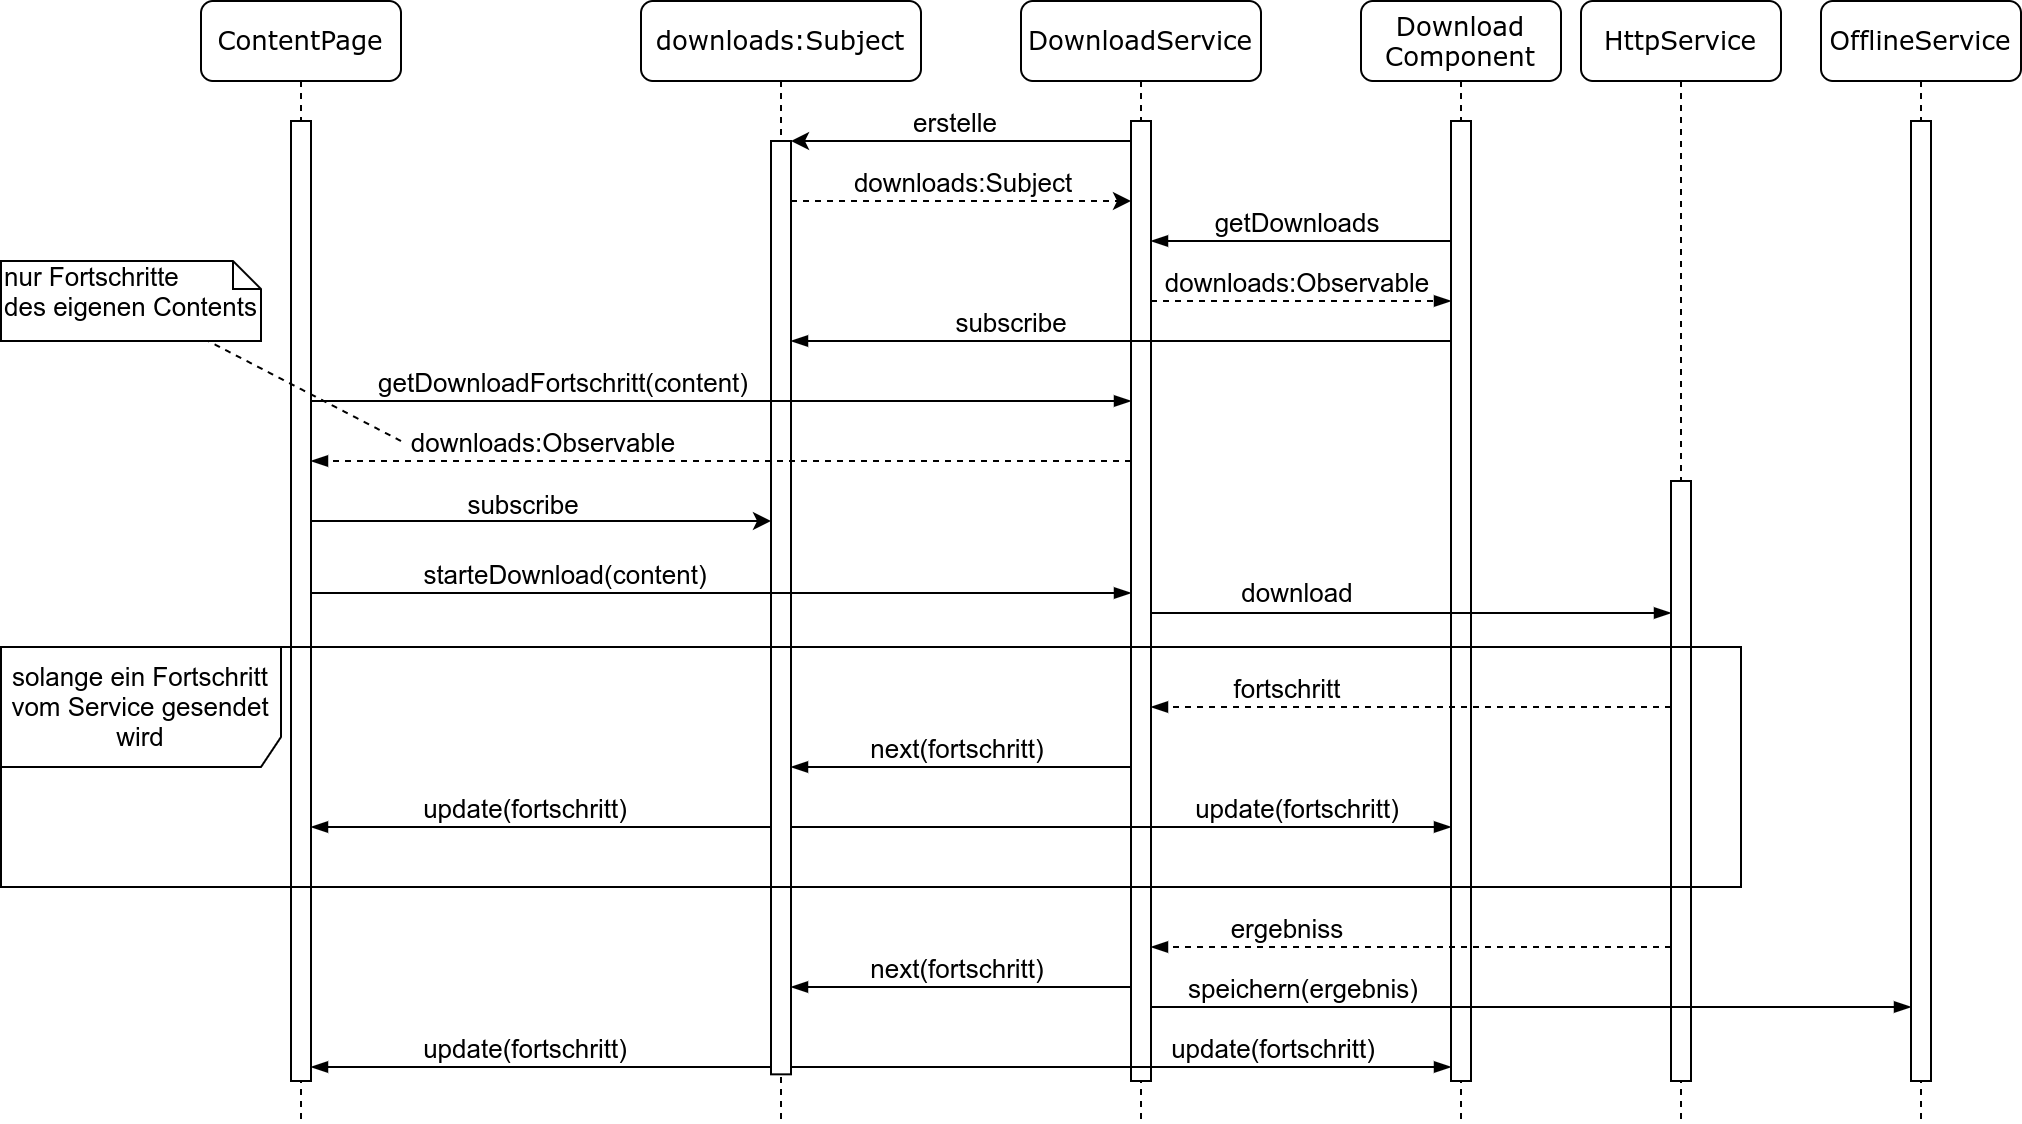
\includegraphics[width=22cm]{diagramme/download-sequenzdiagramm}
  \caption{Sequenzdiagramm für den Download von Dateien}
  \label{diagramme/download-sequenzdiagramm}
\end{sidewaysfigure}

\section{Grafische Oberfläche}
Der Designentwurf für die Funktion \textit{unterwegs anhören} wurde gemeinsam diskutiert und herausgearbeitet. 

In der Desktop-Ansicht wird in den Player ein Switch hinzugefügt, mit dem ein Inhalt offline verfügbar gemacht werden kann. In \autoref{designs/player} ist dieser Player mit dem Button zu sehen. Außerdem gibt es einen Button \textit{Meine Inhalte}, mit dem man auf die Übersichtsseite mit allen heruntergeladenen Inhalten kommt.

\bild{designs/player}{14cm}{Player der Desktop-Ansicht}

Da der Player in der mobilen Ansicht nicht genügend Platz bietet, wird der Switch zum Herunterladen unter dem Player dargestellt. Dies ist in \autoref{designs/player-mobile} zu sehen. Wenn der Player vergrößert wird, erscheint auch der Button \textit{Meine Inhalte} wie in \autoref{designs/player-mobile-gross} zu sehen.

\bild{designs/player-mobile}{8cm}{Design: Player der mobilen Ansicht}

\bild{designs/player-mobile-gross}{8cm}{Design: ausgefahrener Player der mobilen Ansicht}

Zuletzt zeigt \autoref{designs/uebersicht} eine Liste mit allen Inhalten, die heruntergeladen wurden. Diese können einzeln oder alle auf einmal gelöscht werden. Außerdem ist es möglich, einen Inhalt abzuspielen oder alle heruntergeladenen Inhalte zu durchsuchen.

\bild{designs/uebersicht}{8cm}{Design: Liste mit allen heruntergeladenen Inhalten} % Externe Datei einbinden
\chapter{Evaluation und Reflexion}
\label{Kap6}
In diesem Kapitel wird die Arbeit kritisch reflektiert. Welche Anforderungen konnten erfüllt werden und wo gibt es noch Verbesserungspotenzial?

\section{Kann durch die PWA eine native APP ersetzt werden?}
Moderne Webtechnologien können in vielen Fällen eine eigene Native App für Android, iOS oder andere Systeme ersetzten. Ob dies für CROSSLOAD auch der Fall ist, wird in diesem Kapitel untersucht. Dabei wird nur die Offline-Funktionalität berücksichtigt.

Durch das Überprüfen aller Anforderungen aus \autoref{Kap3:Anforderungen} kann festgestellt werden, ob eine \ac{PWA} für CROSSLOAD ausreichend ist oder nicht. Im Nachfolgenden wird jede Anforderung einzeln bewertet. Folgende Bewertungen wurden hierfür festgelegt:
\begin{itemize}
\item erfüllt: Die Anforderung ist ohne Einschränkungen erfüllt
\item teilweise erfüllt: Teile der Anforderung können erfüllt werden oder die Anforderung kann nur in manchen Browsern erfüllt werden
\item nicht erfüllt: Es ist mit einer \ac{PWA} nicht möglich, diese Anforderung zu erfüllen
\end{itemize}

Wenn durch die Verwendung einer nativen App Vorteile für den Nutzer entstehen würden, werden diese auch genannt. \autoref{Anforderungen-Tabelle} zeigt diesen Vergleich.

\begin{sidewaystable}[h]
  \renewcommand{\arraystretch}{1.2}
  \centering
  \sffamily
  \begin{footnotesize}
    \begin{tabularx}{1.0\textwidth}{X l X X}
      \toprule
      \textbf{Anforderung} & \textbf{Erfüllt} & \textbf{Anmerkung} & \textbf{Verbesserung durch native App} \\
      \midrule
      \emph{1: Ein Inhalt kann favorisiert werden} & erfüllt & - & - \\
      \emph{2: Herunterladen eines Inhalts anhand der Verbindungsart} & teilweise & Die Verbindungsart kann nicht in allen Browsern ausgelesen werden & In einer nativen App können alle Netzwerkinformationen ausgelesen werden \\
      \emph{3: Fortschrittsanzeige des Downloads} & erfüllt & - & - \\
      \emph{4: Erkennung eines Verbindungsabbruches} & erfüllt & - & - \\
      \emph{5: Übersicht aller heruntergeladenen Inhalte} & erfüllt & - & - \\
      \emph{6: Sortierung und Filterung aller heruntergeladenen Inhalte} & erfüllt & Eine performante Volltextsuche ist nicht möglich & In einer nativen App ist auch eine performante Volltextsuche möglich \\
      \emph{7: Heruntergeladene Inhalte können gelöscht werden} & erfüllt & - & - \\
      \emph{8: Herausfinden, ob ein bestimmter Inhalt offline verfügbar ist} & erfüllt & - & - \\
	  \emph{9: Metadaten zu einem Inhalt speichern} & erfüllt & - & - \\   
	  \emph{10: Anhören des heruntergeladenen Inhalts} & erfüllt & - & Eine native App würde hier den Vorteil einer konfigurierbaren Benachrichtigung bieten. Über diese Benachrichtigung könnte man dann die Predigt stoppen oder zum nächsten Inhalt springen. \\   
      \emph{11: Eine Audiodatei ist bis zu 100 \ac{MB} groß} & erfüllt & - & - \\
      \emph{12: Die Metadaten zu einem Inhalt sind bis zu 50 \ac{kB} groß} & erfüllt & - & - \\
      \emph{13: Möglichst viele Inhalte speichern} & erfüllt & - & Der verfügbare Speicher im Browser ist begrenzt und nutzt nicht die ganze Festplatte. Bei sehr geringem freien Speicher könnte eine native App mehr Inhalte speichern \\
      \emph{14: Download im Hintergrund} & erfüllt & - & Es gibt in einer \ac{PWA} Einschränkungen, die eine native App nicht hat: Das Browserfenster muss geöffnet bleiben wenn ein Download stattfindet. Durch die Verwendung von Background Fetch, was aber nur in Chrome verfügbar ist, wird dieser Nachteil wieder ausgeglichen. \\
      \bottomrule
    \end{tabularx}
  \end{footnotesize}
  \rmfamily
  \caption{Erfüllung der Anforderungen}
  \label{Anforderungen-Tabelle}
\end{sidewaystable}

\clearpage

Bis auf die Anforderung 2 konnten alle Anforderungen erfüllt werden. Eine native App bietet in vielen Fällen eine bessere Nutzererfahrung, ist aber für die reine Funktionalität nicht notwendig. Für CROSSLOAD ist eine \ac{PWA} eine gute Alternative zu einer nativen App. Der Aufwand, für jede Plattform eine eigene App zu schreiben, ist nicht angemessen, um Anforderung 2 für alle Nutzer zu erfüllen. Außerdem verbessert sich die Unterstützung neuer \acp{API} kontinuierlich in allen Browsern. Dadurch ist zu erwarten, dass die Einschränkungen in Anforderung 2 in Zukunft nicht mehr vorhanden sein werden.

\section{Nutzerfreundlichkeit}
Generell bieten die neuen Offline-Funktionen, welche in dieser Thesis entwickelt wurden, einen Mehrwert für die Nutzer. Wie intensiv die Funktionen genutzt werden, wird sich jedoch erst in den nächsten Monaten in der Praxis zeigen. 

Es gibt einen Punkt, der noch zu verbessern ist und wofür noch keine gute Lösung gefunden wurde. Die hier entwickelten Offline-Funktionalitäten speichern Audio\-dateien im Browser in einer Datenbank. Auf CROSSLOAD gibt es aber auch die Möglichkeit, die Audiodatei als mp3-Datei auf das Endgerät herunterzuladen. Die heruntergeladene mp3-Datei kann dann zum Beispiel an andere Personen per Mail oder Bluetooth verschickt werden. Andererseits hat das Speichern im Browser den Vorteil der Übersichtlichkeit: Alle verfügbaren Inhalte sind direkt einsehbar und auch verwaltbar. Weil beide Funktionen Vorteile haben, sollen beide Funktionen erhalten bleiben. Für den Nutzer ist es auf den ersten Blick jedoch sehr schwer zu verstehen, was der Unterschied der beiden Optionen (offline verfügbar machen und herunterladen) ist. Für diesen Zweck wurde eine Erklärseite eingeführt, die dem Nutzer diese Funktion erklärt, wenn er sich dafür interessiert. Es könnte jedoch das Problem auftreten, dass viele Nutzer diese Erklärung nicht lesen und deswegen die neuen Offline-Funktionalitäten nicht kennenlernen und davon profitieren können. 

Deswegen ist es sehr wichtig, das Verhalten der Nutzer auf der Seite zu analysieren und gegebenenfalls eine andere Möglichkeit zu finden, dem Nutzer die neuen Offline-Funktionalitäten zu erklären.
 % Externe Datei einbinden
\chapter{Zusammenfassung und Ausblick}
\label{Kap7}
Dieses Kapitel gibt eine Zusammenfassung der ganzen Arbeit. Zuletzt werden auch noch einige Punkte genannt, die in Zukunft angedacht werden könnten, um CROSSLOAD weiter zu verbessern.

\section{Zusammenfassung}
Das Ziel dieser Arbeit war es, das bereits vorhandene Webportal CROSSLOAD um eine Offline-Funktionalität zu erweitern. Außerdem wurde dabei untersucht, welche Webtechnologien dafür zur Verfügung stehen und ob diese ausreichen, um alle Anforderungen zu erfüllen. Dem Nutzer soll es möglich sein, Inhalte des Portals im Browser zu speichern und diese Inhalte auch nutzen zu können, wenn keine oder eine schlechte Internetverbindung besteht. Moderne Browser bieten die Möglichkeit, Daten in einer Datenbank der IndexedDB zu speichern, die auch ein Filtern und Durchsuchen erlaubt. In dieser Datenbank werden Inhalte und deren Metadaten gespeichert. Der Download der Inhalte findet in einem Angular Service statt. Es gibt andere Technologien, wie Background Fetch, die dem Nutzer eine bessere Erfahrung bieten würden, diese sind aber nicht für alle Browser verfügbar. Zum Bereitstellen der Inhalte und des Downloadfortschrittes wird immer auf das Publish-Subscribe Pattern gesetzt. Dadurch ist es sehr flexibel möglich, Daten an mehrere Komponenten weiterzugeben. Die grafische Oberfläche für diese Funktionen wurde noch nicht fertig entwickelt, sondern nur die Machbarkeit des Vorhabens gezeigt. Entwürfe für das endgültige Design sind für spätere Entwicklungen vorhanden. Zusammenfassend kann gesagt werden, dass Webtechnologien und \acp{PWA} sehr gut geeignet sind, um dem Nutzer auch eine Offline-Nutzung zu ermöglichen. Fast alle Anforderungen konnten ohne Kompromisse umgesetzt werden. Nur eine Anforderung ist noch nicht in allen Browsern umsetzbar. Die Entwicklung wird dadurch erschwert, dass nicht jeder Browser alle Funktionen implementiert. Dazu gehört zum Beispiel die Möglichkeit, die Verbindungsart wie WLAN oder mobile Daten auszulesen, um den Download von Inhalten zu steuern. Außerdem bieten \acp{PWA} noch nicht ausreichend die Möglichkeit, Berechnungen im Hintergrund auszuführen. Ein Download von Inhalten im Hintergrund, während der Browser also geschlossen, beziehungsweise minimiert ist, ist deswegen nicht auf allen Geräten möglich. Diese Funktionalität kann einigen Nutzern zur Verfügung gestellt werden, eine Alternative für nicht unterstützte Geräte muss aber trotzdem entwickelt werden. Wie die neuen Funktionalitäten vom Nutzer angenommen werden, ist noch zu beobachten und aufgrund dieser Erkenntnisse ist es wichtig, das Portal immer wieder anzupassen.

\section{Ausblick}
Nach dem Abschluss dieser Arbeit gibt es noch viele Möglichkeiten, CROSSLOAD zu verbessern. Dazu gehört zuerst die Implementierung der erarbeiteten Designs. Die Designs müssen auch regelmäßig überdacht und evaluiert werden und dementsprechend das Portal angepasst werden. Außerdem ist eine Sortierung, Filterung und das Durchsuchen der Offline-Inhalte noch nicht implementiert. Dies ist vor allem für Nutzer mit sehr vielen Inhalten nützlich. 

Beim Beobachten einiger Nutzer ist aufgefallen, dass Inhalte schnell heruntergeladen werden aber dann vergessen werden, zu löschen. Dies führt dann dazu, dass der Speicher knapp wird und eventuell sogar dazu, dass keine neuen Inhalte mehr heruntergeladen werden können. Dafür könnte eine Strategie entwickelt werden, wann Inhalte automatisch gelöscht werden. Alternativ kann dem Nutzer selbst die Möglichkeit gegeben werden einzustellen, wann Inhalte automatisch gelöscht werden sollen. Das könnte in verschiedene Kriterien wie \textit{wurde die Predigt schon angehört} oder \textit{wann wurde der Inhalt heruntergeladen} unterteilt werden. Anhand dieser Kriterien kann eine Bewertung erstellt werden, wie relevant der Inhalt noch für den Nutzer ist. Die Inhalte mit der geringsten Bewertung werden gelöscht, sobald Speicher benötigt wird.

Zuletzt sollte eine Synchronisation der heruntergeladenen Inhalte über mehrere Geräte entwickelt werden. Ein Nutzer möchte seine Inhalte vielleicht auf dem Laptop auswählen und dann unterwegs auf seinem Smartphone anhören. Der Nutzer legt sich dafür einen Account bei CROSSLOAD an oder meldet sich über einen anderen Dienst wie Google oder Facebook bei CROSSLOAD an. Die vorgemerkten Inhalte werden dann auf einem Server von CROSSLOAD für jeden Nutzer gespeichert. Bei jedem Start des Portals, auf dem Smartphone oder Laptop, wird die Liste der vorgemerkten Inhalte geladen und gegebenenfalls neue Inhalte heruntergeladen. 
 % Externe Datei einbinden
% ------------------------------------------------------------------

\label{lastpage}

% Neue Seite
\cleardoublepage

% Backmatter mit normalem Zeilenabstand setzen
\singlespacing

% Römische Ziffern für die "Back-Matter", fortlaufend mit "Front-Matter"
\pagenumbering{roman}
\setcounter{page}{\value{frontmatterpage}}

% Glossar
\addchap{\hsmaglossar}
\glsaddallunused
\setglossarysection{section}
\printglossary[title=Glossar]

% Abkürzungsverzeichnis
\addchap{\hsmaabbreviations}
% Die längste Abkürzung kann in die eckigen Klammern
% bei \begin{acronym} geschrieben, um einen hässlichen
% Umbruch zu verhindern
%
% ACHTUNG: Sie müssen die Abkürzungen von Hand alphabetisch
%          sortieren. Das passiert nicht automatisch.
\begin{acronym}[PWA]
\acro{API}{Application Programming Interface}
\acro{MB}{Megabyte}
\acro{PWA}{Progressive Web App}
\end{acronym}


% Abbildungsverzeichnis erzeugen
\cleardoublepage
\phantomsection
\addcontentsline{toc}{chapter}{\hsmalistoffigures}
\listoffigures

% Tabellenverzeichnis erzeugen
\cleardoublepage
\phantomsection
\addcontentsline{toc}{chapter}{\hsmalistoftables}
\listoftables

% Listingverzeichnis erzeugen. Wenn Sie keine Listings haben,
% entfernen Sie einfach diesen Teil.
% \cleardoublepage
% \phantomsection
% \addcontentsline{toc}{chapter}{\hsmalistings}
% \lstlistoflistings

% Literaturverzeichnis erzeugen
\begingroup
\cleardoublepage
\begin{flushleft}
\let\clearpage\relax % Fix für leere Seiten (issue #25)
\printbibliography
\end{flushleft}
\endgroup

% Index ausgeben. Wenn Sie keinen Index haben, entfernen Sie einfach
% diesen Teil. Die meisten Abschlussarbeiten haben *keinen* Index.
%\cleardoublepage
%\phantomsection
%\addcontentsline{toc}{chapter}{\hsmaindex}
%\printindex

% Anhang. Wenn Sie keinen Anhang haben, entfernen Sie einfach
% diesen Teil.
% \appendix
% \chapter{Erster Anhang}

Hier ein Beispiel für einen Anhang. Der Anhang kann genauso in Kapitel und Unterkapitel unterteilt werden, wie die anderen Teile der Arbeit auch.

% \chapter{Zweiter Anhang}

Hier noch ein Beispiel für einen Anhang.


\end{document}
